\documentclass{article}

%change margins
\usepackage[a4paper, left=2cm, right=2cm, top=2.5cm, bottom=2.5cm]{geometry}
%placement accuracy
\usepackage{float}
% Needed for custom title page
\usepackage{titling} 
\usepackage{array}
%for figures
\usepackage{graphicx}
\usepackage{subcaption}

%for coding highlighting
\usepackage{listings}
\usepackage{xcolor}

\usepackage{multirow} % Required for multirow cells
\usepackage{amsmath} % Required for math equations

% Font and language setup (XeLaTeX only)
\usepackage{fontspec}
\usepackage{polyglossia}
\setdefaultlanguage{greek}
\setotherlanguage{english}

\setmainfont{Palatino Linotype}
\newfontfamily\greekfont{Palatino Linotype} % Optional: redefine Greek font explicitly
\newfontfamily\greekfonttt{FreeMono}


\lstdefinestyle{cppstyle}{
    language=C++,
    basicstyle=\ttfamily\footnotesize,
    keywordstyle=\color{blue},
    commentstyle=\color{gray},
    stringstyle=\color{teal},
    backgroundcolor=\color{white},
    frame=single,
    breaklines=true,
    breakatwhitespace=false,
    tabsize=4,
    showstringspaces=false,
    captionpos=b
}
% NOTE: We're already using polyglossia for Greek text support
% and fontspec has already been loaded above
\setmainfont{Times New Roman}

\title{\Huge Ιεραρχία Μνήμης}
\author{
  \textbf{Χαράλαμπος Παπαδόπουλος\\ 03120199} \\[3cm]
  {Προηγμένα Θέματα Αρχιτεκτονικής Υπολογιστών\\ 2η Άσκηση} \\
}
\date{Μάιος 2025}


\begin{document}

\begin{titlepage}
    \centering
    \vspace{3cm}

    
\includegraphics[width=4cm]{figures/emp.png}\\
    \vspace{1.5cm}
    {\fontsize{24pt}{20pt}\selectfont{Εθνικό Μετσόβιο Πολυτεχνείο}}\\[0.3cm]
    {\fontsize{16pt}{18pt}\selectfont Σχολή Ηλεκτρολόγων Μηχανικών \& Μηχανικών Υπολογιστών}\\[0.3cm]
    {\fontsize{16pt}{18pt}\selectfont Αρχιτεκτονική Υπολογιστών}\\[2cm]

    {\Huge\bfseries \thetitle \par}
    \vspace{2cm}
    {\Large \theauthor \par}
    \vfill

    {\fontsize{15pt}{18pt}Απρίλιος 2025}
\end{titlepage}

\section{Εισαγωγή}
Στην παρούσα εργασία θα μελετήσουμε διάφορες αρχιτεκτονικές μνήμης χρησιμοποιοώντας το εργαλείο προσομοίωσης PIN.

\section{L2 Cache}
Αρχικά, θα εξετάσουμε την επίδραση που έχουν στην επίδοση τα βασικά χαρακτηριστικά της L2, δηλαδή το μέγεθος, η συσχετιστικότητα (associativity) και το μέγεθος του cache block.

Οι συνδυασμοί που θα δοκιμάσουμε είναι οι εξής:

\begin{table}[h!]
\centering
\begin{tabular}{|c|c|c|}
\hline
\textbf{L2 size (KB)} & \textbf{L2 associativity} & \textbf{L2 cache block size (B)} \\
\hline
256 & 4, 8 & \multirow{4}{*}{64, 128, 256} \\
\cline{1-2}
512 & 4, 8 & \\
\cline{1-2}
1024 & 8, 16 & \\
\cline{1-2}
2048 & 16 & \\
\hline
\end{tabular}
\caption{L2 Cache Configuration}
\label{tab:l2cache}
\end{table}

Σημειώνεται πως η πολιτική αντικατάστασης, σε όλες τις περιπτώσεις, είναι LRU (Least Recently Used).

Για την προσομοίωση χρησιμοποιούμε 7 benchmarks από τη σουίτα `SPEC\_CPU2006`. 

Για κάθε cache configuration θα χρησιμοποιοιήσουμε τον γεωμετρικό μέσο όρο των 7 benchmarks προκειμένου να εξάγουμε συπεράσματα.

Οι μετρικές που θα χρησιμοποιήσουμε είναι οι εξής:
\begin{itemize}
    \item \textbf{Instructions per cycle (IPC)}: Μέτρο της απόδοσης ενός επεξεργαστή, που δείχνει τον μέσο αριθμό εντολών που εκτελούνται σε κάθε κύκλο του ρολογιού του επεξεργαστή. Υψηλότερο IPC σημαίνει γενικά καλύτερη απόδοση.
\end{itemize}




\[
\text{Cycles} = \text{Instructions} + (\mathit{L1\_Accesses} \times \mathit{L1\_hit\_cycles}) + (\mathit{L2\_Accesses} \times \mathit{L2\_hit\_cycles}) + (\mathit{Mem\_Accesses} \times \mathit{Mem\_acc\_cycles})
\]


\begin{itemize}
\item \textbf{Επιτυχία στην κρυφή μνήμη L1}: 1 κύκλος\\
(\( \mathit{L1\_hit\_cycles} = 1 \))
\item \textbf{Επιτυχία στην κρυφή μνήμη L2}: 15 κύκλοι\\
(\( \mathit{L2\_hit\_cycles} = 15 \))
\item \textbf{Πρόσβαση στην κύρια μνήμη}: 250 κύκλοι\\
(\( \mathit{Mem\_acc\_cycles} = 250 \))
\end{itemize}

Για την εκτέλεση των προσομοιώσεων τροποποιήσαμε το αρχείο `run\_benchmarks.sh`.
Συγκεκριμένα, τροποποιήσαμε την παράμετρο
$\mathit{CONFS} = \texttt{"256\_4\_64 256\_4\_128 256\_4\_256 256\_8\_64 256\_8\_128 \dots}"$ 
προκειμένου να περιλαμβάνει τα configurations που ζητούνται.

Λαμβάνουμε, λοιπόν, τα εξής αποτελέσματα:

\begin{figure}[H]
    \centering
    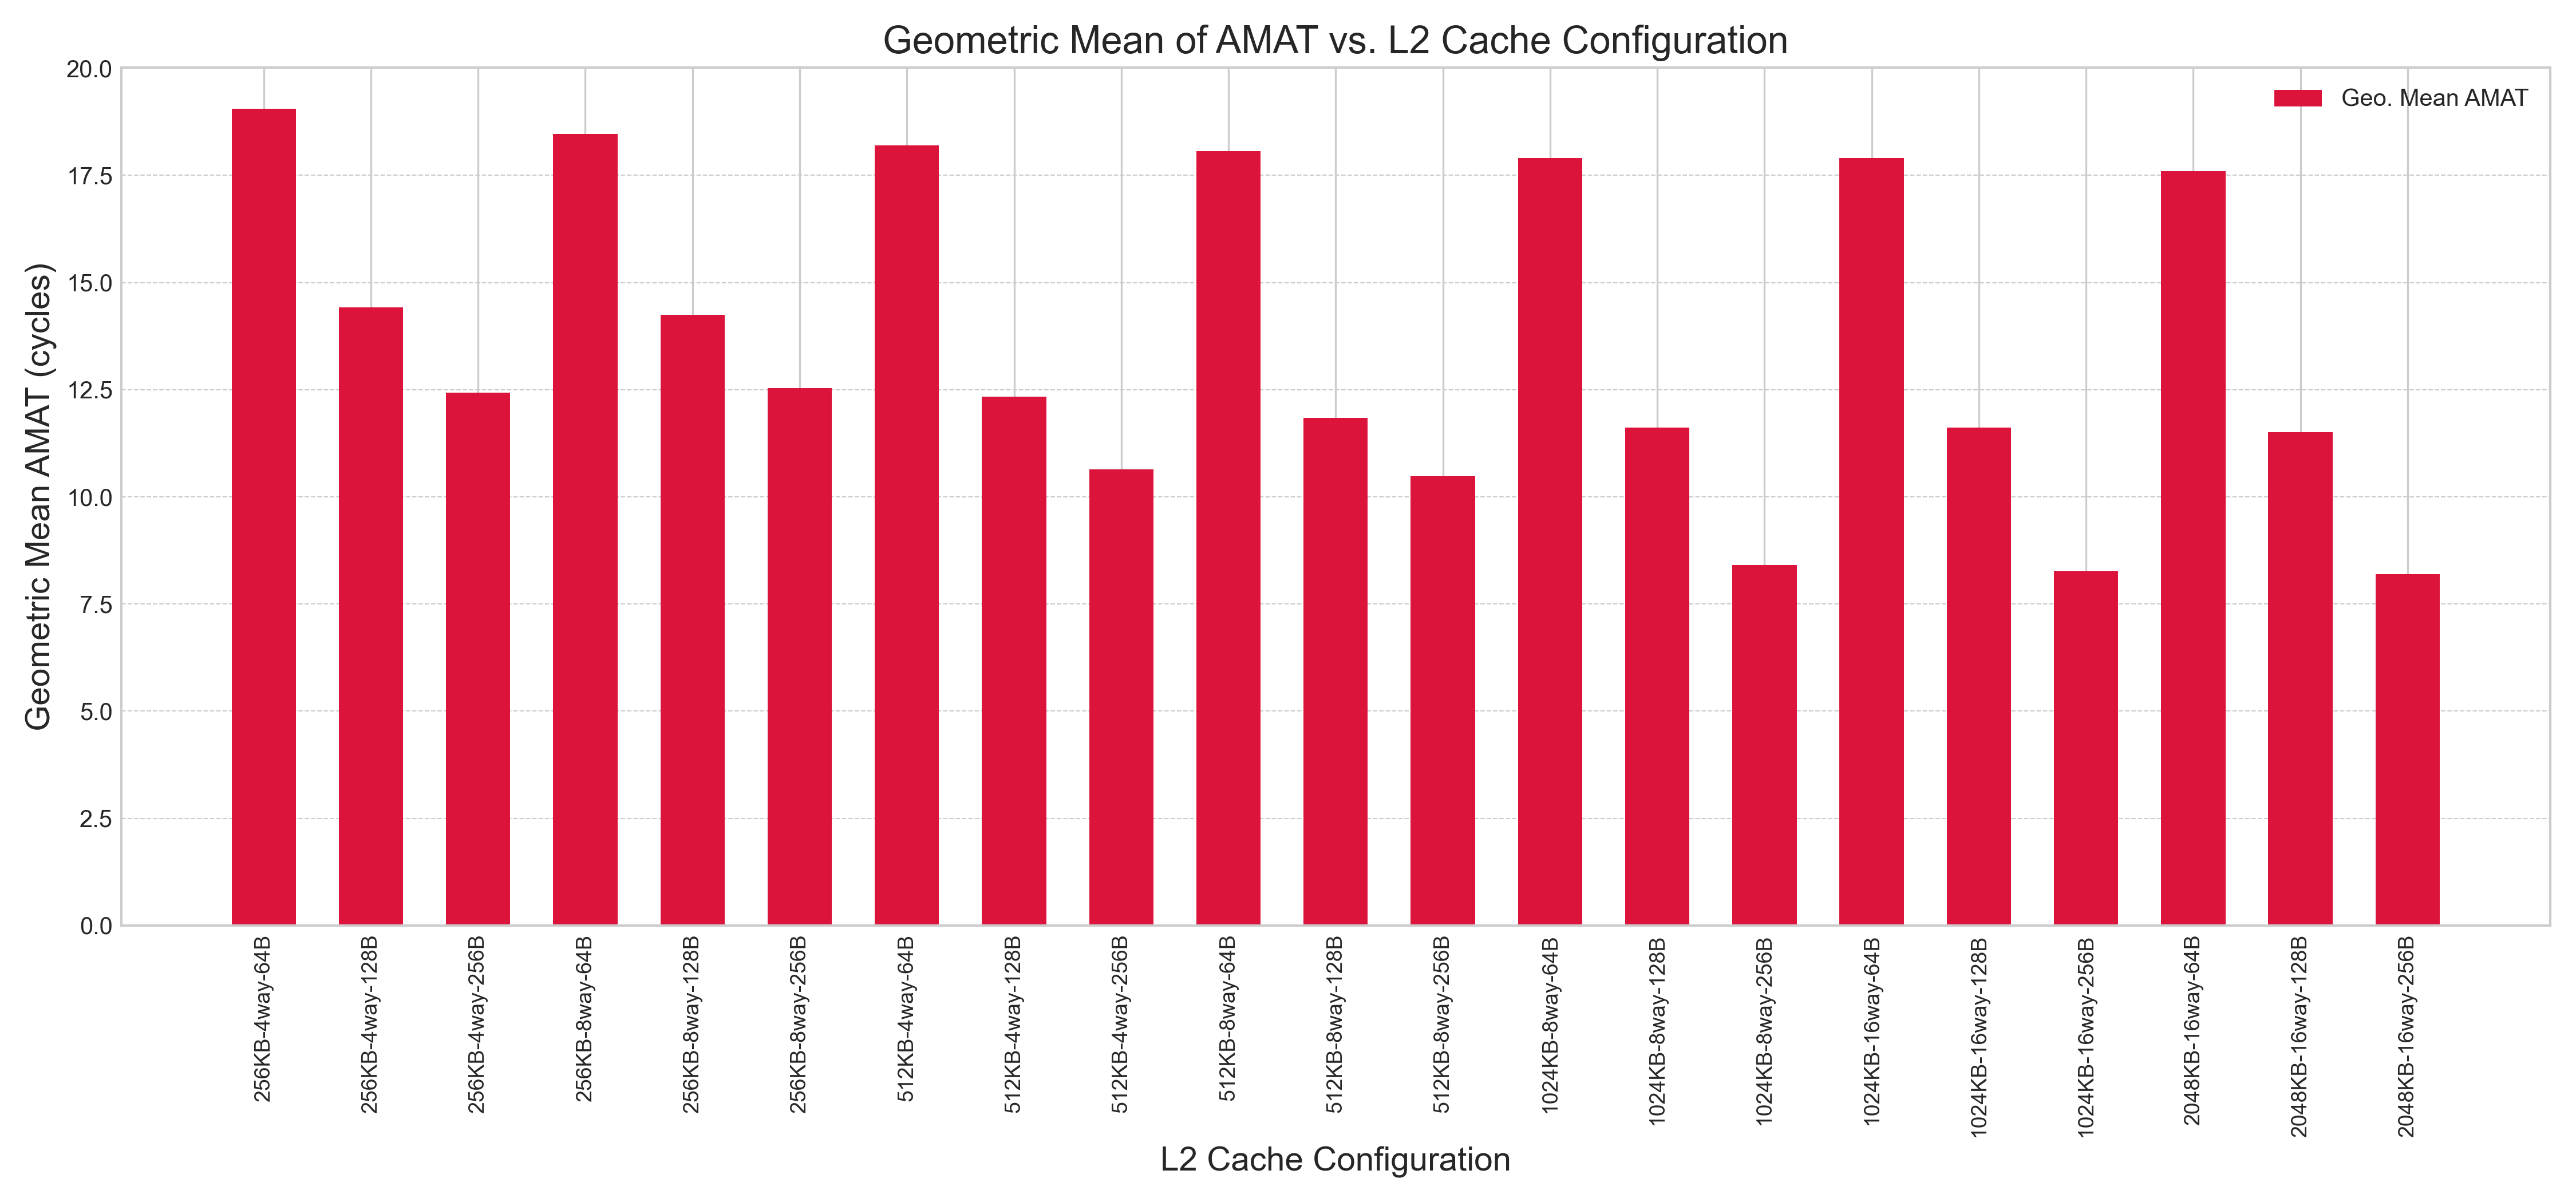
\includegraphics[width=\textwidth]{figures/lru/amat_lru.png}
    \caption{L2 Cache Configuration Results}
    \label{fig:l2cache_amat}
\end{figure}

\begin{figure}[H]
    \centering
    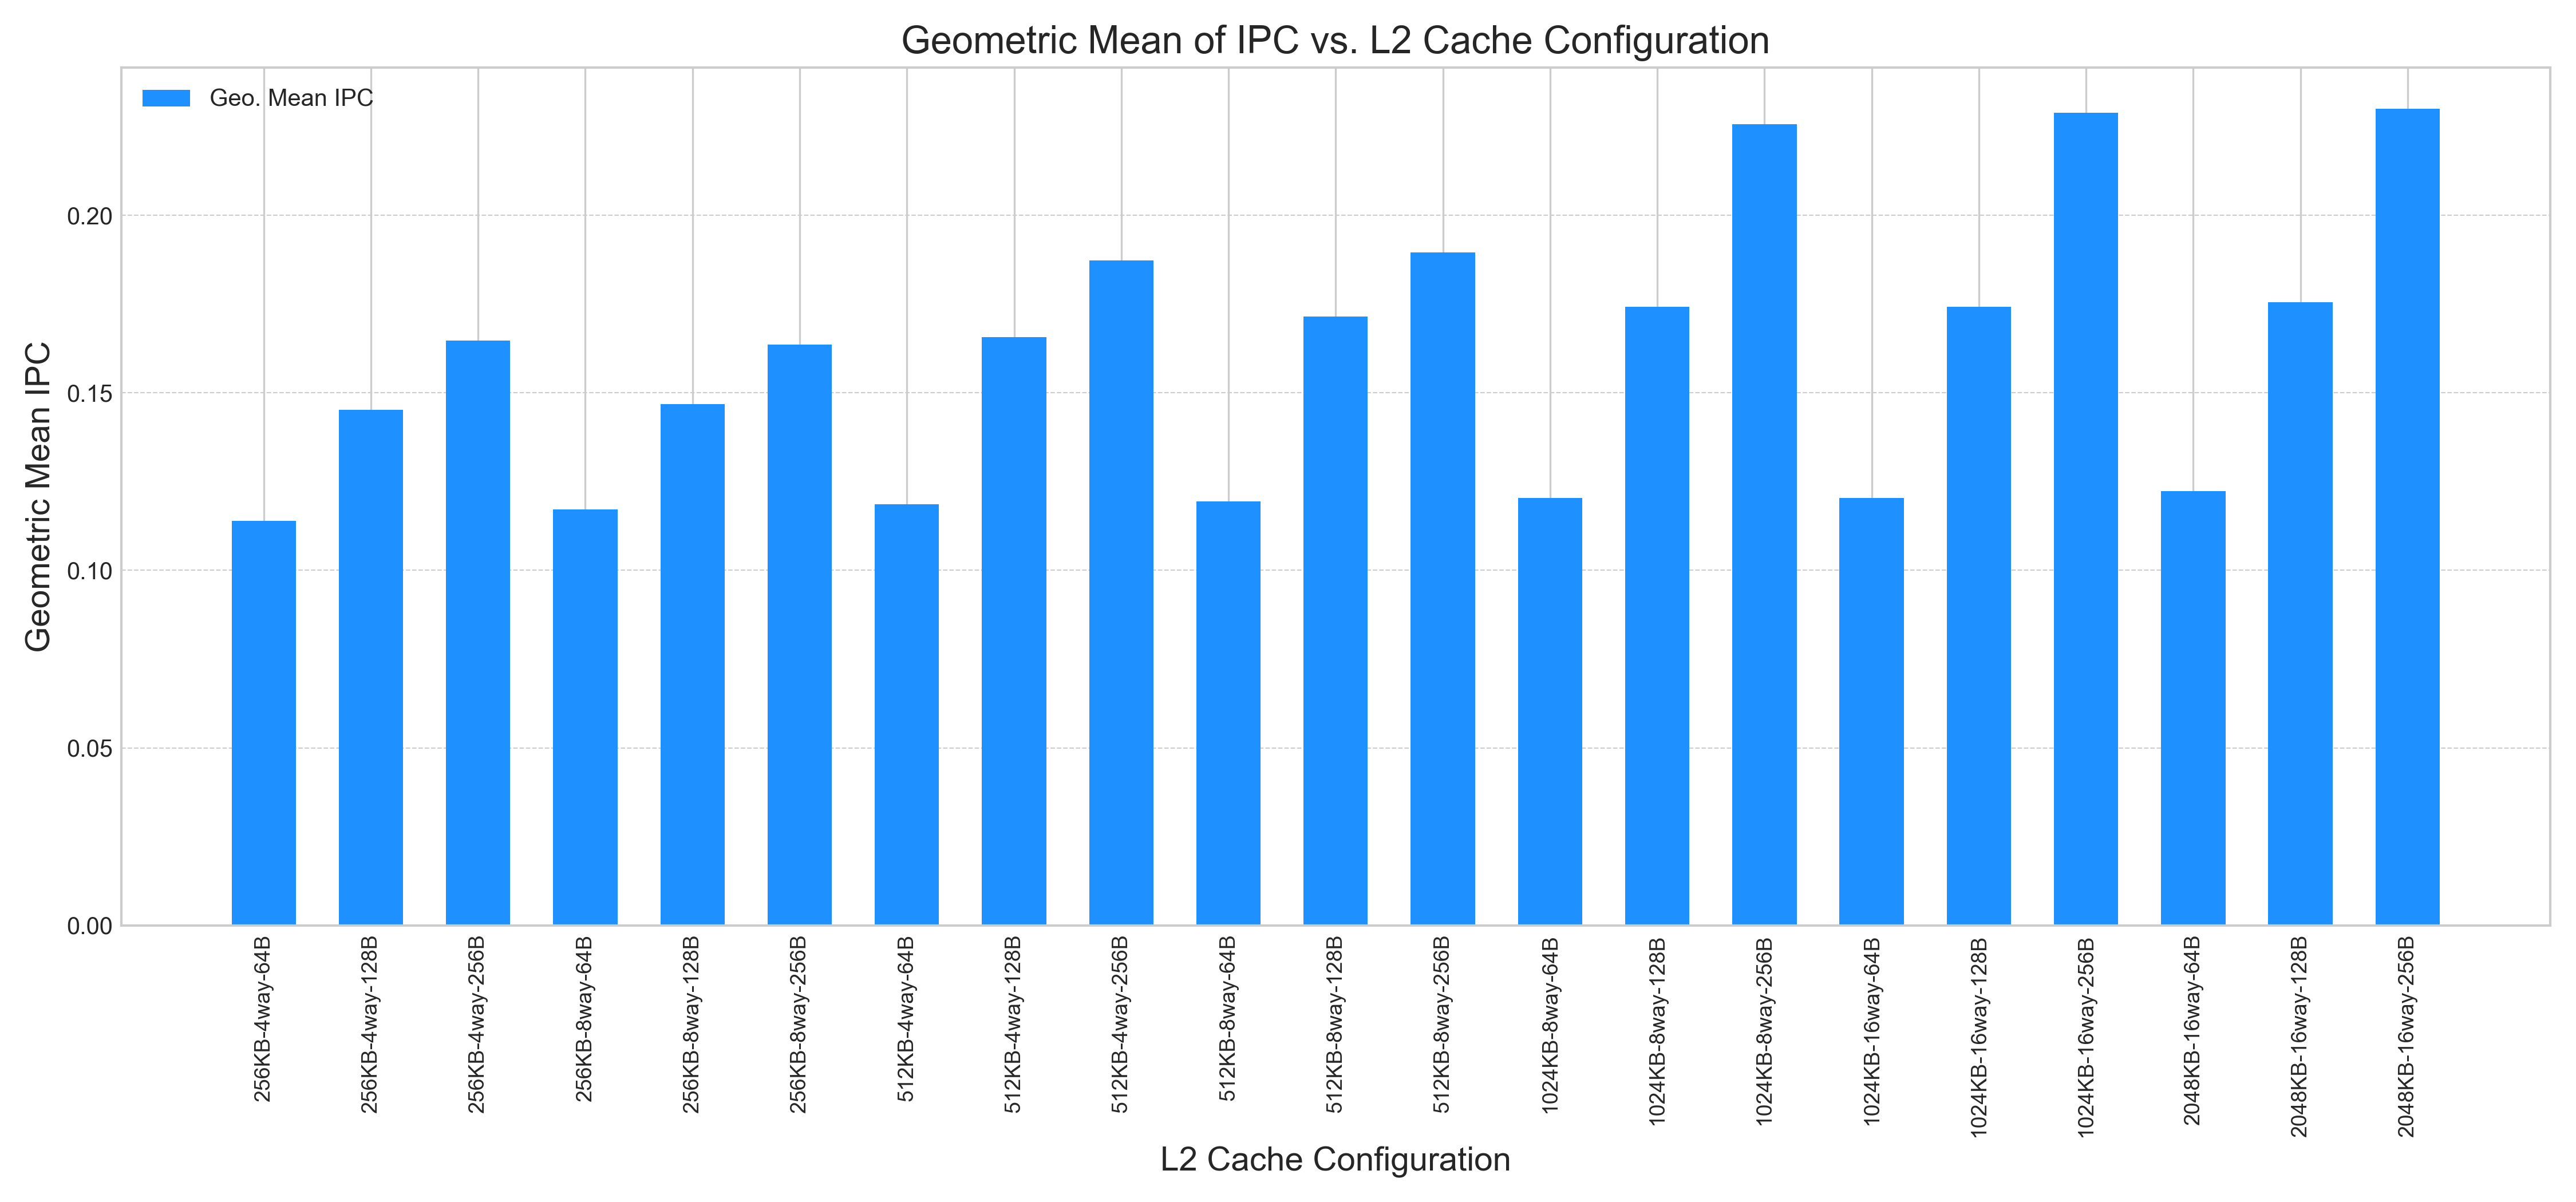
\includegraphics[width=\textwidth]{figures/lru/ipc_lru.png}
    \caption{L2 Cache Configuration Results}
    \label{fig:l2cache_ipc}
\end{figure}

\begin{figure}[H]
    \centering
    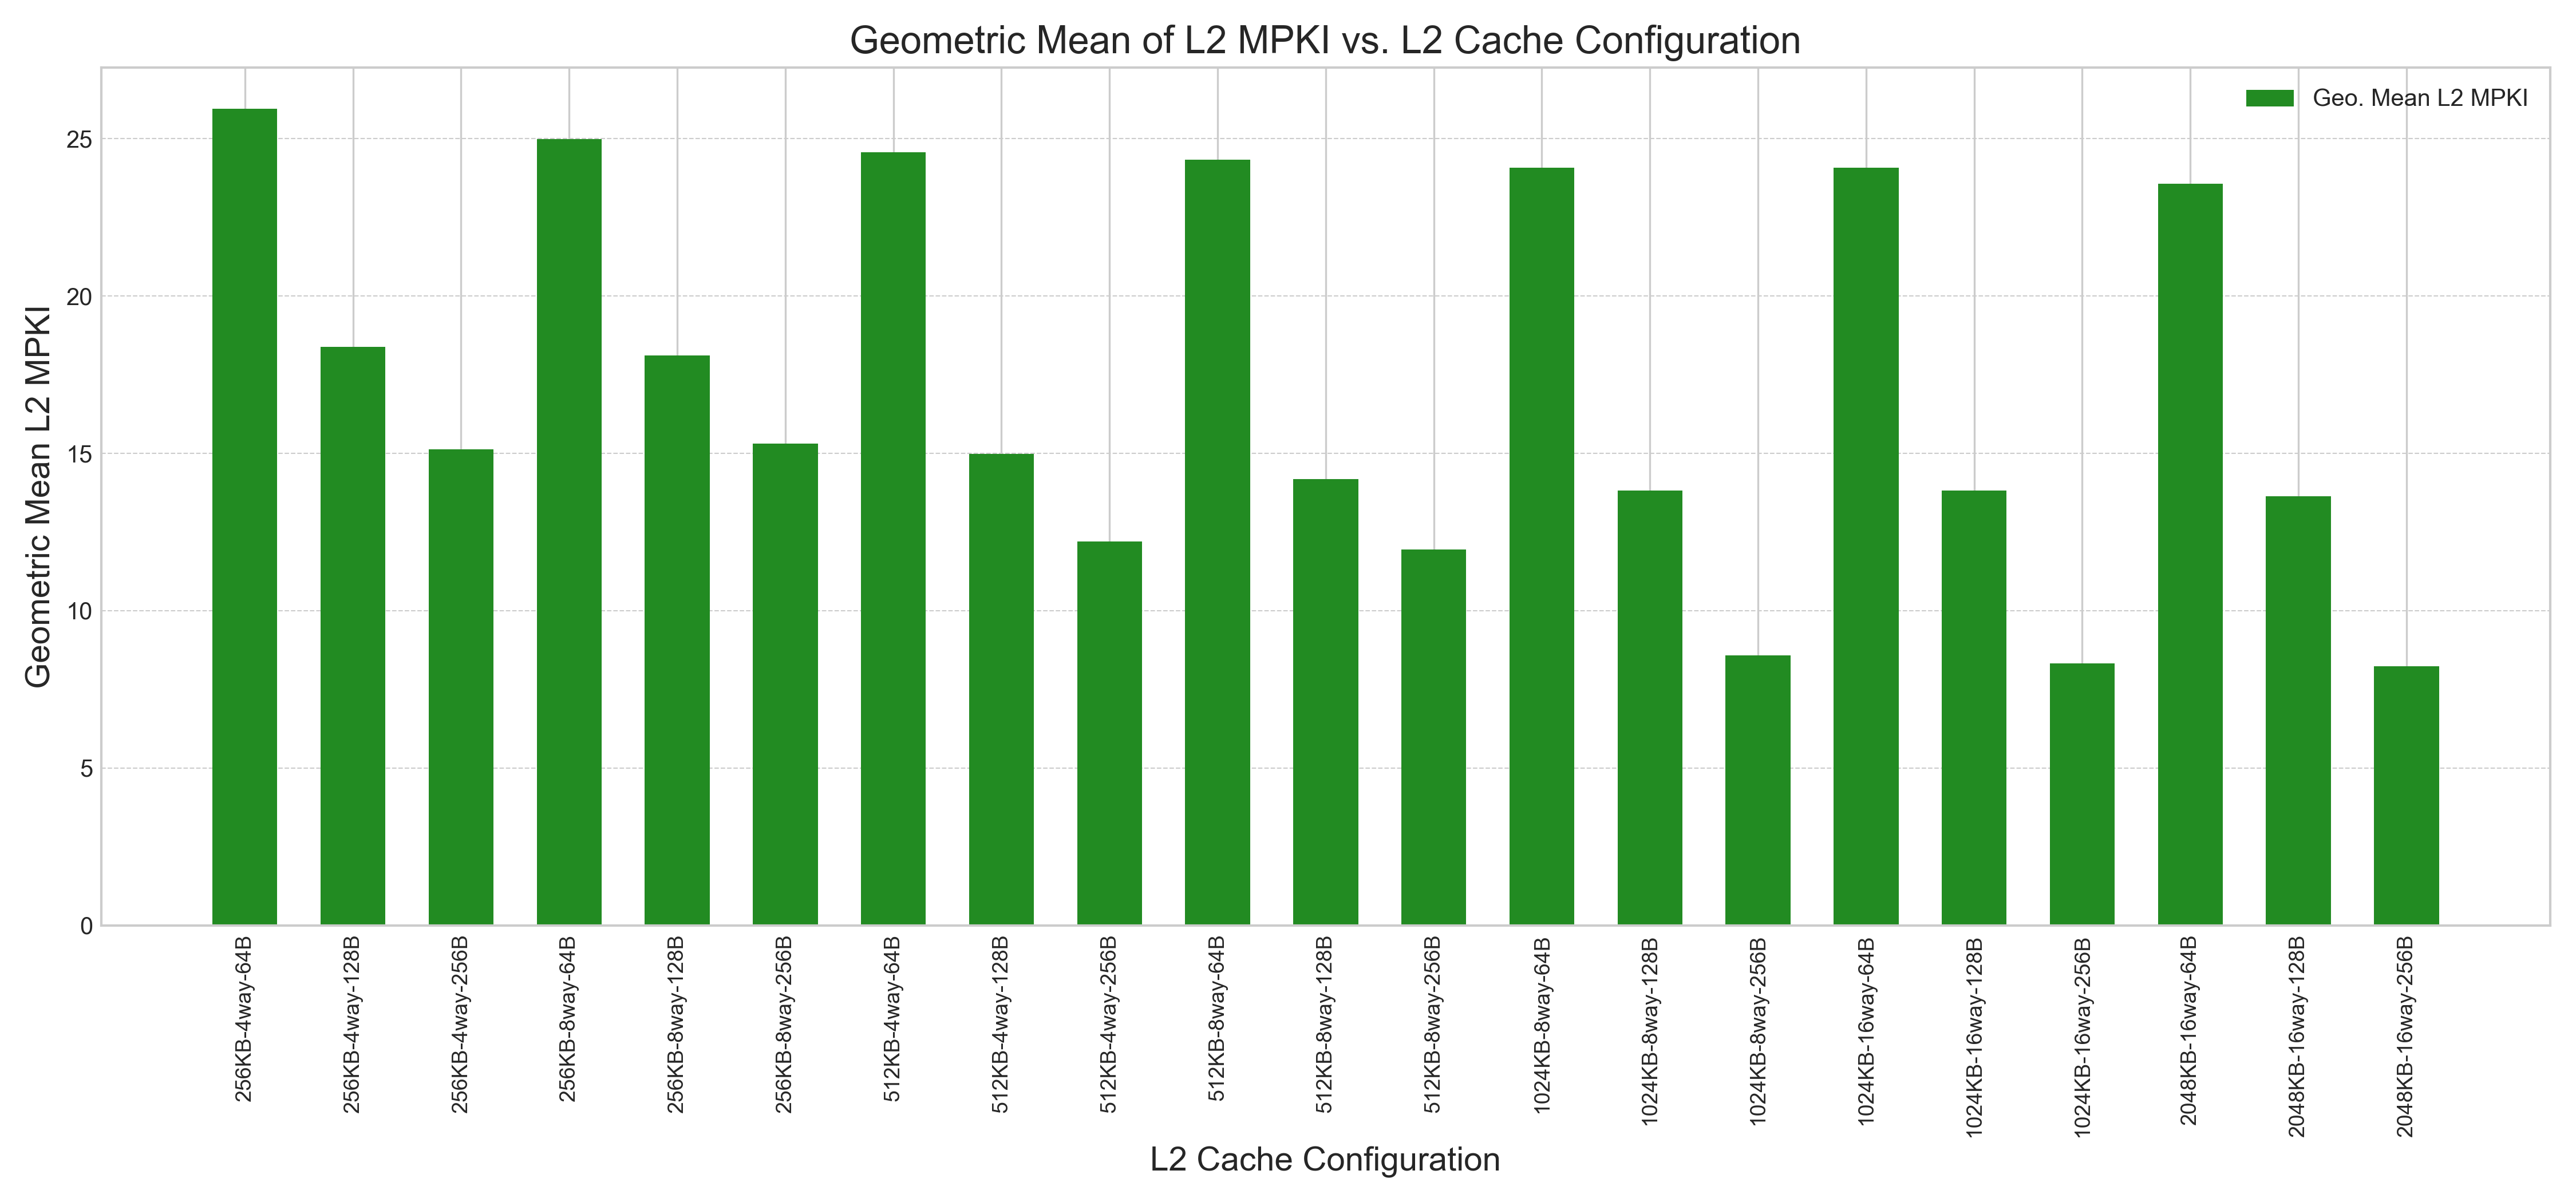
\includegraphics[width=\textwidth]{figures/lru/mpki_lru.png}
    \caption{L2 Cache Configuration Results}
    \label{fig:l2cache_lru}
\end{figure}


Βάσει των αποτελεσμάτων προσομοίωσης, οι 4 κορυφαίες διαμορφώσεις κρυφής μνήμης L2:

\begin{itemize}
    \item \textbf{Κρυφή μνήμη L2 $2048KB$, $16-way$ associativity, μέγεθος block $256B$}
    \begin{itemize}
        \item $IPC$: Υψηλότερο (περίπου $0.225$)
        \item $AMAT$: Χαμηλότερος (περίπου $8.2$ κύκλοι)
        \item L2 $MPKI$: Χαμηλότερο (περίπου $8.0$)
    \end{itemize}
    Αυτή η διαμόρφωση επιδεικνύει την καλύτερη συνολική απόδοση σε όλες τις βασικές μετρικές.

    \item \textbf{Κρυφή μνήμη L2 $1024KB$, $8-way$ associativity, μέγεθος block $256B$}
    \begin{itemize}
        \item $IPC$: Δεύτερο υψηλότερο (περίπου $0.22$)
        \item $AMAT$: Πολύ χαμηλός (περίπου $8.4$ κύκλοι)
        \item L2 $MPKI$: Πολύ χαμηλό (περίπου $8.5$)
    \end{itemize}
    Αυτή η διαμόρφωση προσφέρει απόδοση πολύ κοντά στην κορυφαία διαμόρφωση με μικρότερο μέγεθος κρυφής μνήμης.

    \item \textbf{Κρυφή μνήμη L2 $1024KB$, $16-way$ associativity, μέγεθος block $256B$}
    \begin{itemize}
        \item $IPC$: Τρίτο υψηλότερο (περίπου $0.215$)
        \item $AMAT$: Πολύ χαμηλός (περίπου $8.4$ κύκλοι)
        \item L2 $MPKI$: Πολύ χαμηλό (περίπου $8.5$)
    \end{itemize}

    \item \textbf{Κρυφή μνήμη L2 $512KB$, $8-way$ associativity, μέγεθος block $256B$}
    \begin{itemize}
        \item $IPC$: Υψηλό (περίπου $0.19$)
        \item $AMAT$: Χαμηλός (περίπου $10.5$ κύκλοι)
        \item L2 $MPKI$: Χαμηλό (περίπου $12.0$)
    \end{itemize}
    Ακόμη και με μικρότερη χωρητικότητα $512KB$, αυτή η διαμόρφωση με $8-way$ associativity και μέγεθος block $256B$ παρέχει ισχυρό $IPC$ και καλά χαρακτηριστικά πρόσβασης μνήμης, καθιστώντας την κορυφαία επιλογή μεταξύ των μικρότερων επιλογών κρυφής μνήμης.
\end{itemize}

Αυτές οι επιλογές δίνουν προτεραιότητα σε υψηλότερες τιμές $IPC$, οι οποίες υποδεικνύουν καλύτερη συνολική απόδοση του επεξεργαστή υπό την παραδοχή σταθερού κύκλου ρολογιού και αριθμού εντολών. 
Αυτές οι διαμορφώσεις παρουσιάζουν επίσης ευνοϊκό (χαμηλότερο) Μέσο Χρόνο Πρόσβασης Μνήμης ($AMAT$) (που επηρεάζεται από τις καθυστερήσεις προσπέλασης) και L2 Αποτυχίες Ανά Χίλιες Εντολές ($MPKI$) ενισχύοντας την αποδοτικότητά τους. 

\section{Πολιτικές Αντικατάστασης}
Στη συνέχεια, θα εξετάσουμε την επίδραση που έχουν στην επίδοση οι πολιτικές αντικατάστασης της L2 cache.
Θα εξετάσουμε τις εξής πολιτικές αντικατάστασης:
\begin{itemize}
    \item \textbf{Random}: Η πολιτική αυτή επιλέγει τυχαία σε κάθε set το block που θα αντικατασταθεί.
    \item \textbf{Least Frequently Used (LFU)}: Η πολιτική Least Frequently Used (LFU) καταγράφει πόσες φορές χρησιμοποιείται κάθε block της cache και όταν χρειαστεί να αντικαταστήσει κάποιο, επιλέγει το block του set που έχει χρησιμοποιηθεί λιγότερο.
    \item \textbf{LRU Insertion Policy (LIP)}: Η πολιτική LIP αποτελεί παραλλαγή της LRU πολιτικής, με μοναδική διαφορά το χαρακτηρισμό των blocks που εισάγονται κάθε φορά στην cache. Συγκεκριμένα, κάθε block που εισάγεται στο set εξαιτίας κάποιου miss, χαρακτηρίζεται ως το LRU block του set (αντί για το MRU, όπως συμβαίνει στην κλασική LRU πολιτική).
    \item \textbf{Static Re-reference Prediction (SRRIP)}: Η πολιτική SRRIP προσπαθεί να αποτρέψει blocks που θα χρησιμοποιηθούν στο μακρινό μέλλον να καταλάβουν πολύτιμο χώρο στην cache. Για να το πετύχει αυτό, εκτιμά πότε θα χρησιμοποιηθεί ξανά κάθε block (θα έχουμε δηλαδή re-reference) και όταν χρειάζεται να αντικαταστήσει κάποιο, επιλέγει το block του set που έχει προβλεφθεί ότι θα χρησιμοποιηθεί στο πιο μακρινό μέλλον. Κάθε block έχει μήκος n bits, όπου n το associativity της cache.
\end{itemize}

Βρίσκουμε, λοιπόν, τα εξής αποτελέσματα:

\begin{figure}[H]
    \centering
    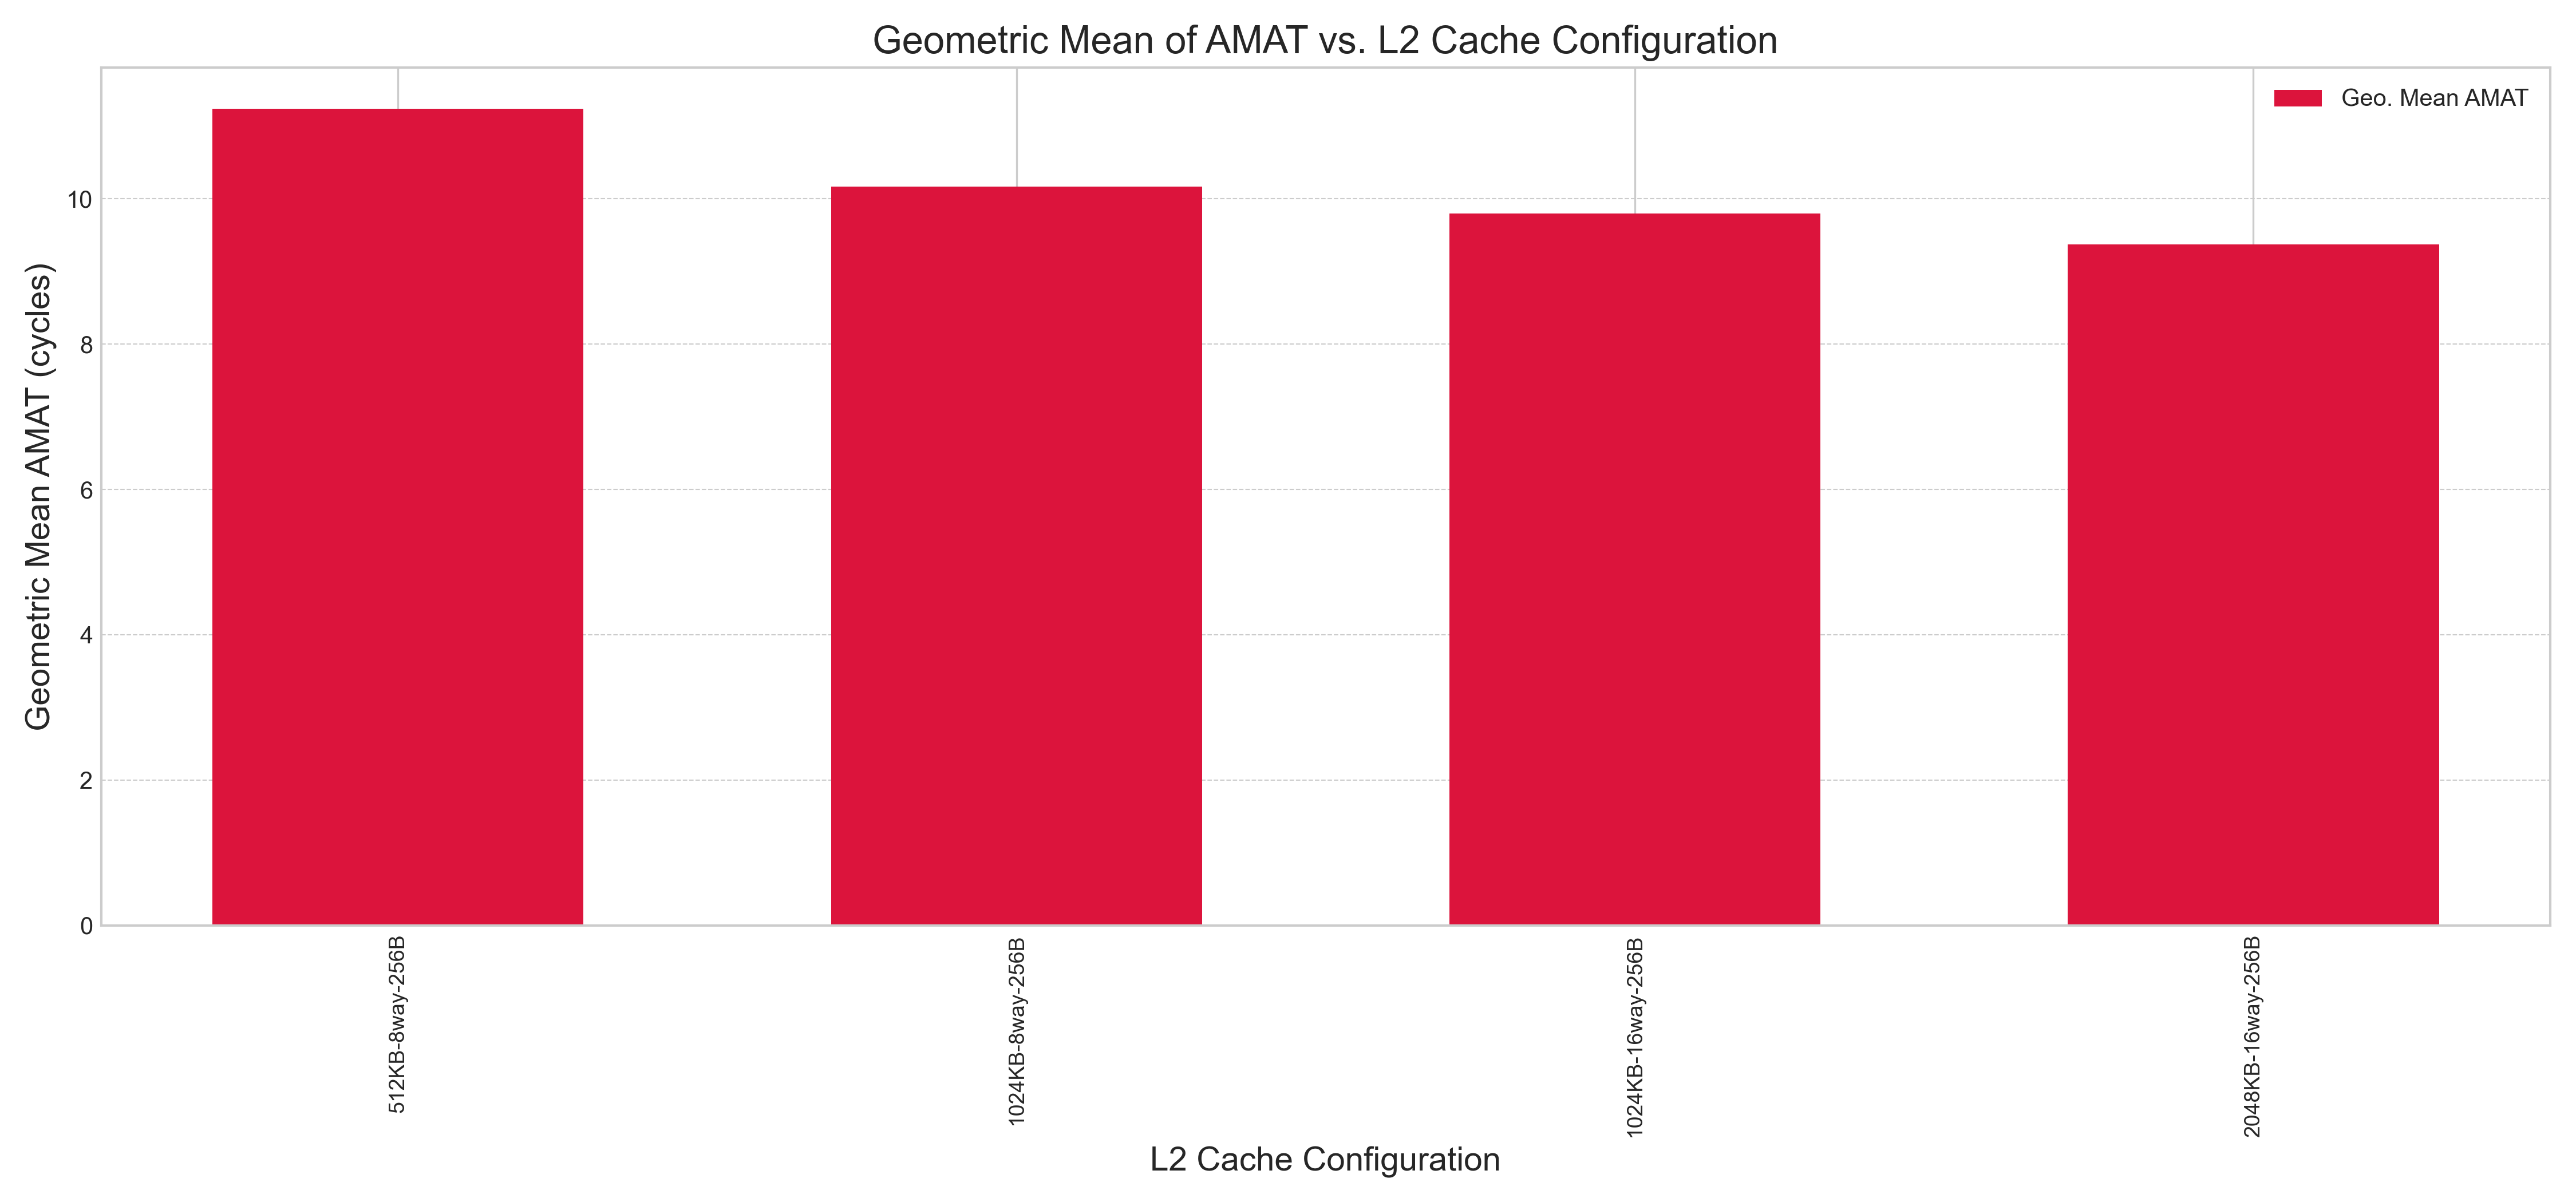
\includegraphics[width=0.8\textwidth]{figures/random/amat_random.png}
    \caption{Random Replacement Policy Results}
    \label{fig:random_amat}
\end{figure}

\begin{figure}[H]
    \centering
    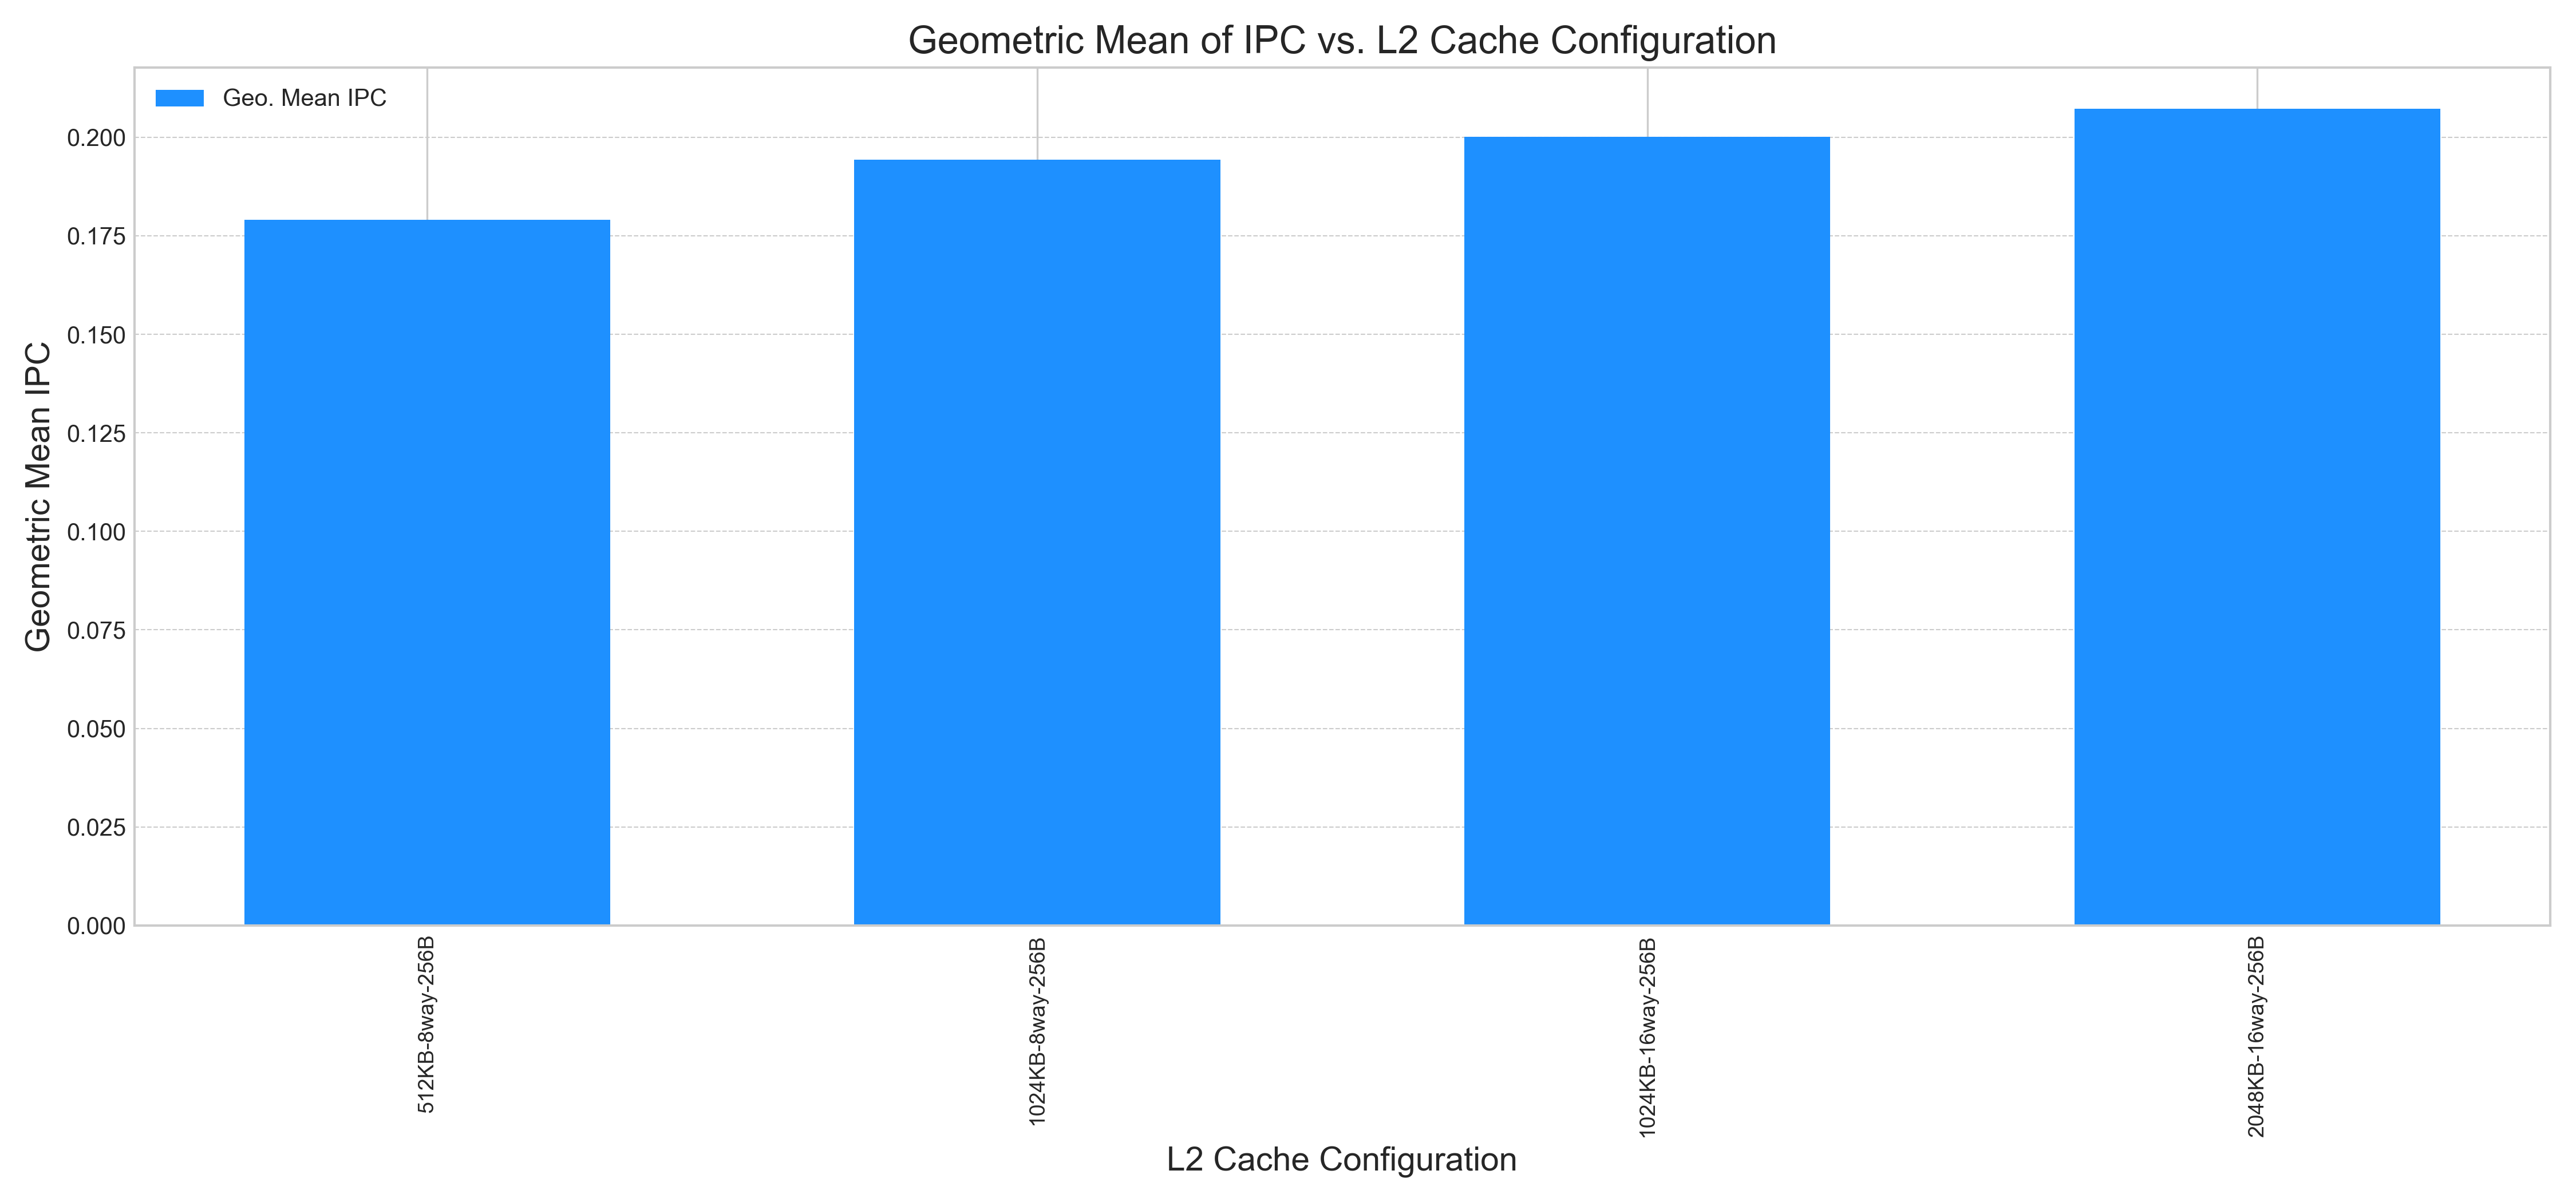
\includegraphics[width=0.8\textwidth]{figures/random/ipc_random.png}
    \caption{Random Replacement Policy Results}
    \label{fig:random_ipc}
\end{figure}

\begin{figure}[H]
    \centering
    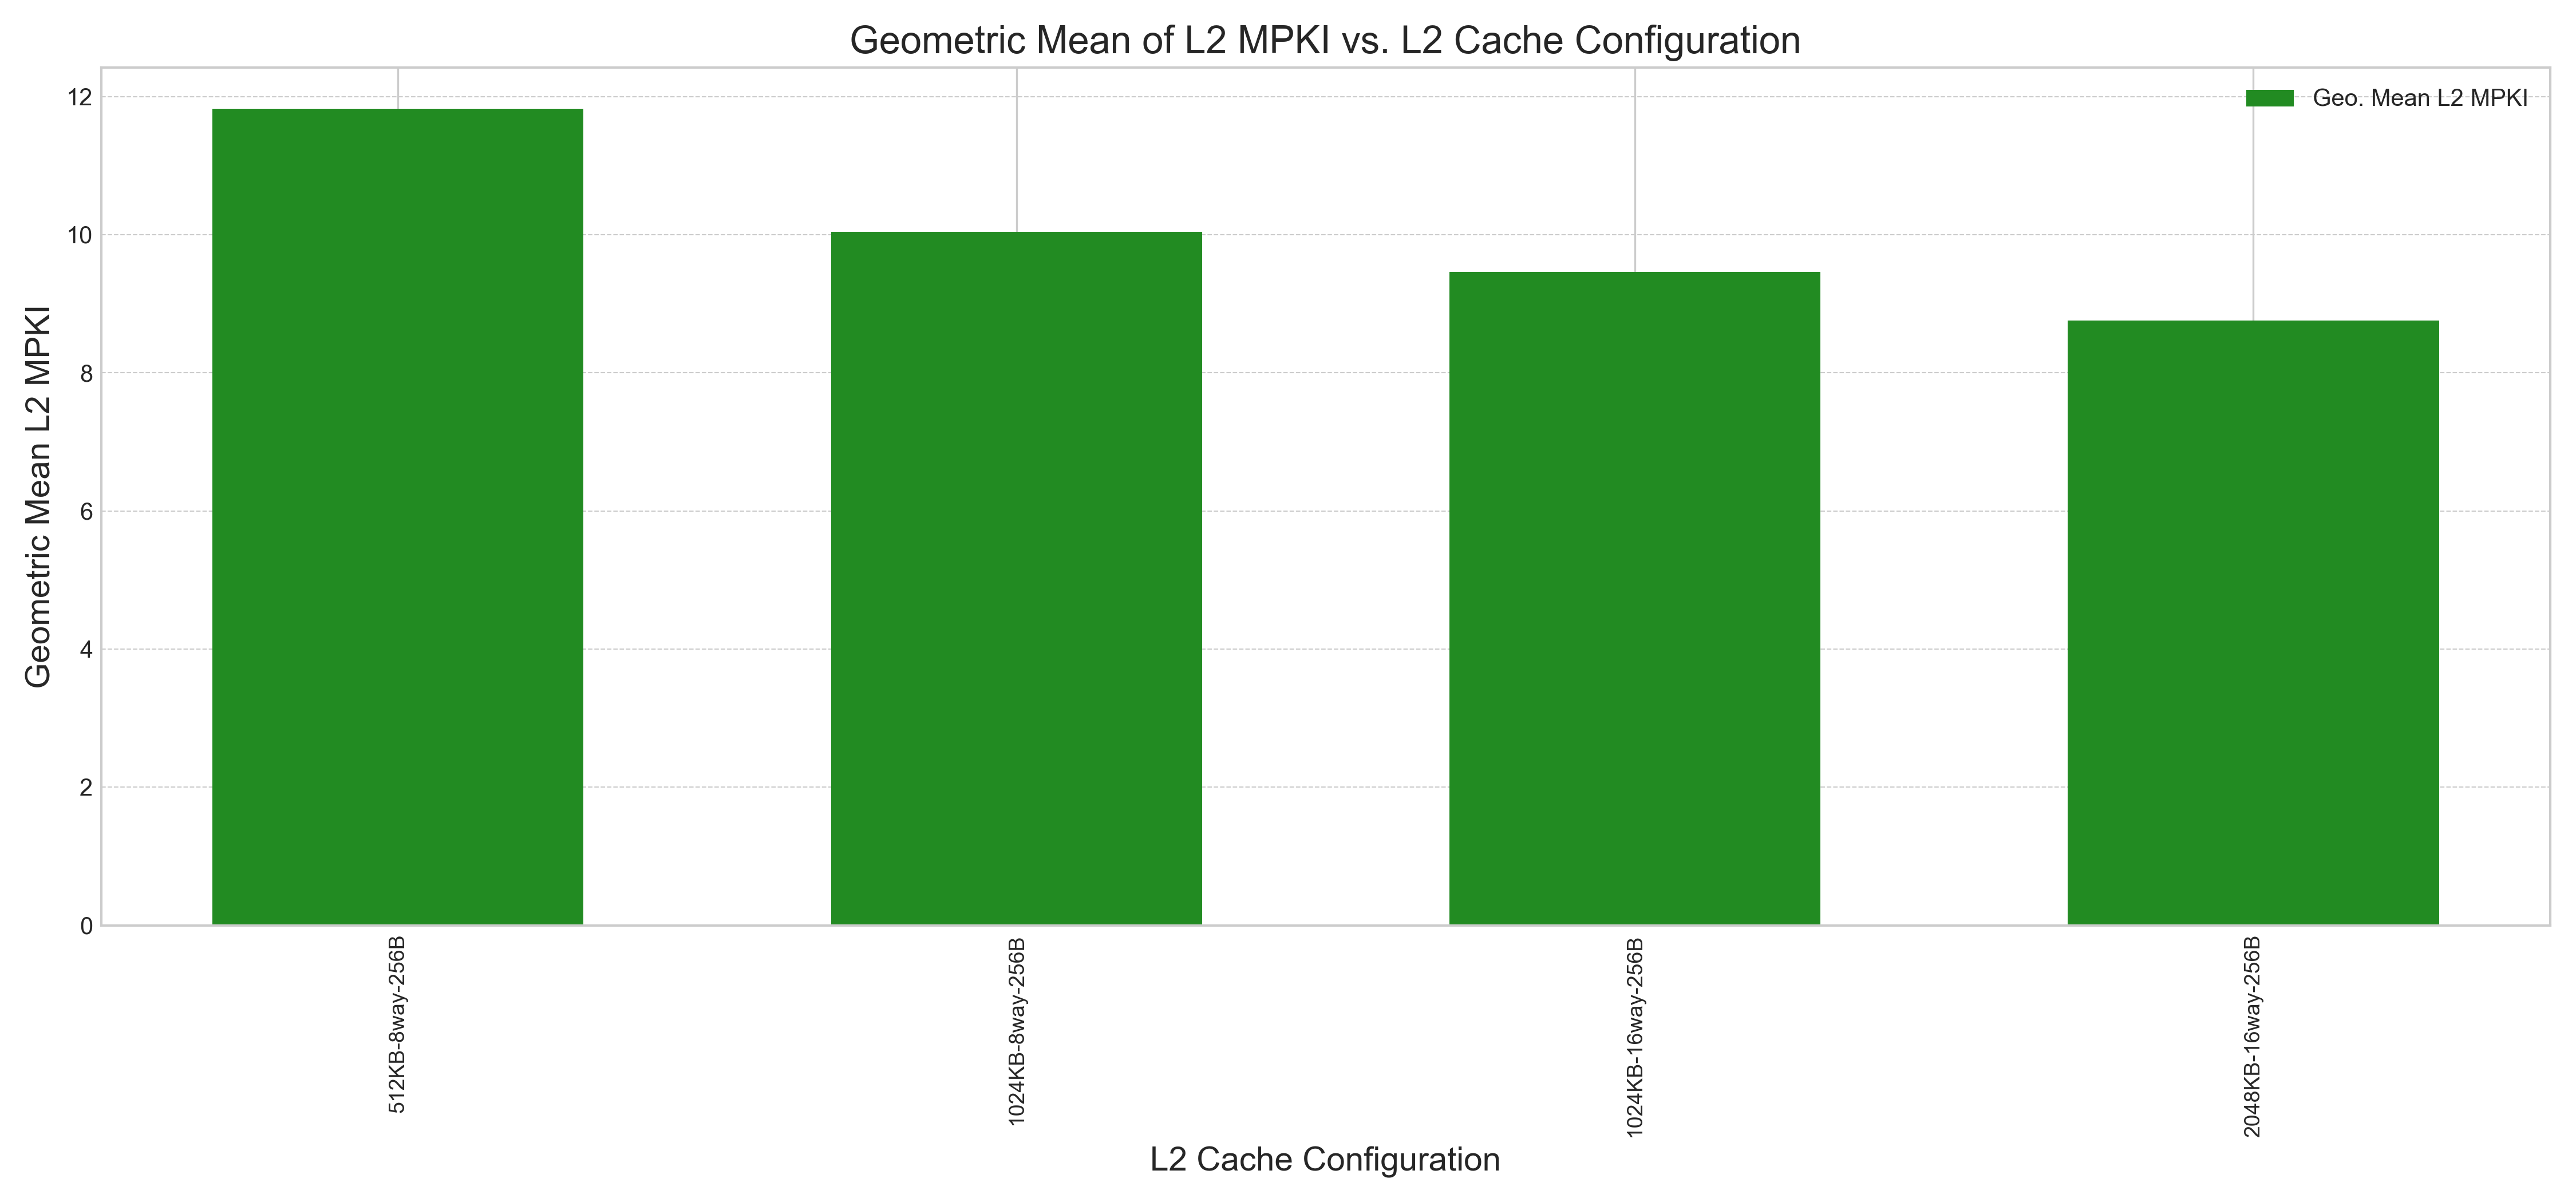
\includegraphics[width=0.8\textwidth]{figures/random/mpki_random.png}
    \caption{Random Replacement Policy Results}
    \label{fig:random_mpki}
\end{figure}

\begin{figure}[H]
    \centering
    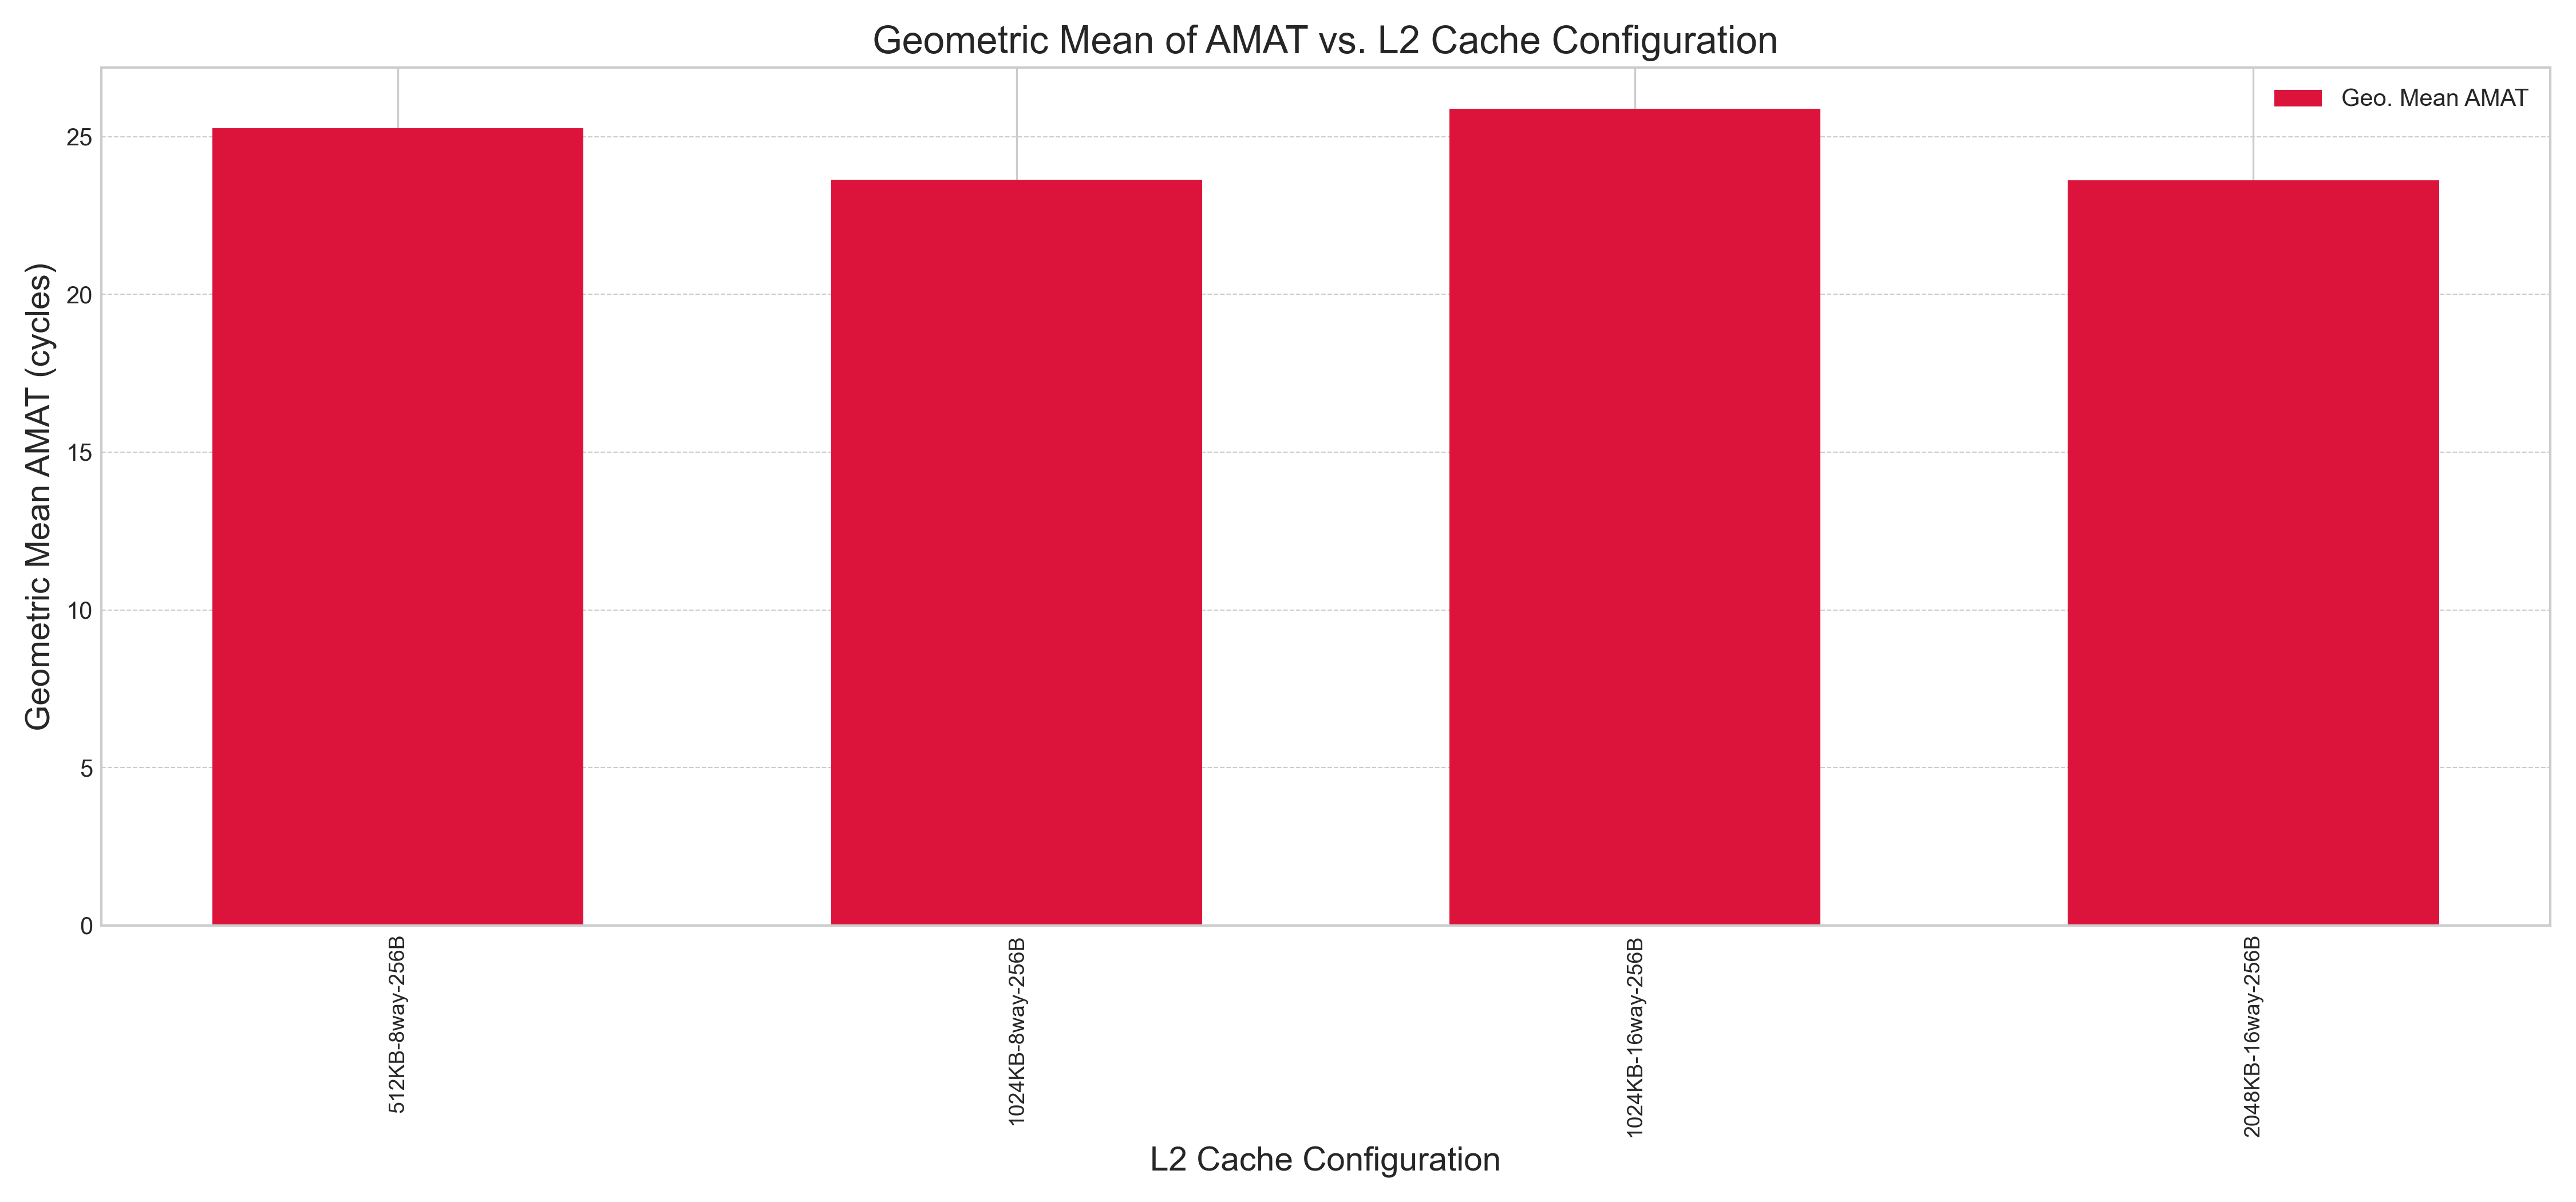
\includegraphics[width=0.8\textwidth]{figures/lfu/amat_lfu.png}
    \caption{LFU Replacement Policy Results}
    \label{fig:lfu_amat}
\end{figure}

\begin{figure}[H]
    \centering
    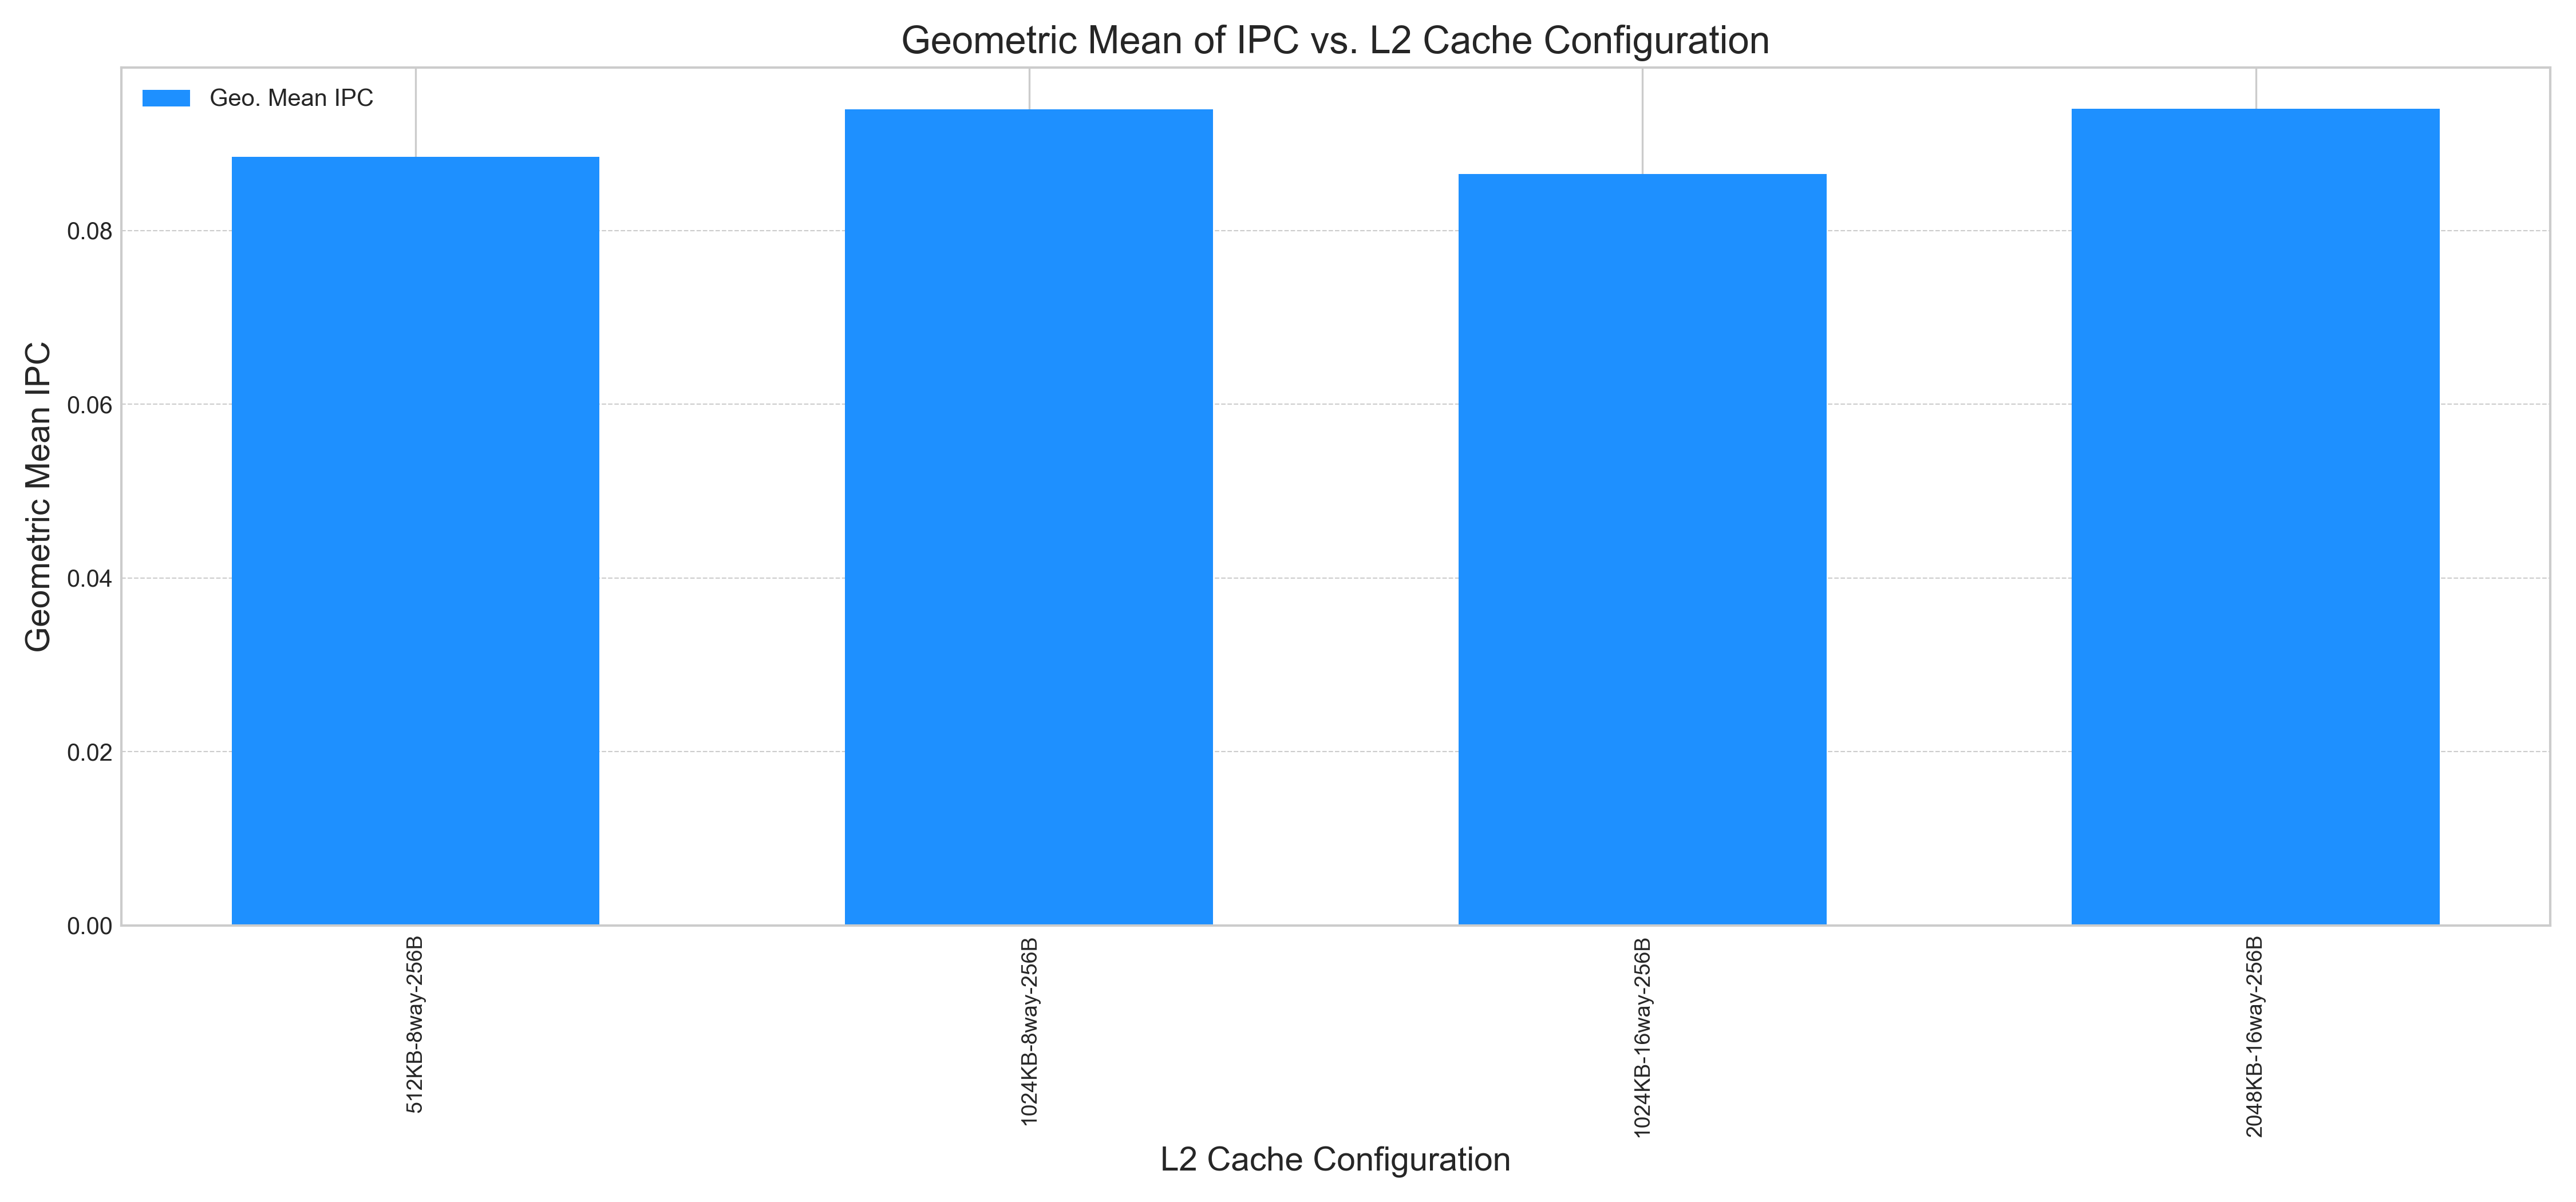
\includegraphics[width=0.8\textwidth]{figures/lfu/ipc_lfu.png}
    \caption{LFU Replacement Policy Results}
    \label{fig:lfu_ipc}
\end{figure}

\begin{figure}[H]
    \centering
    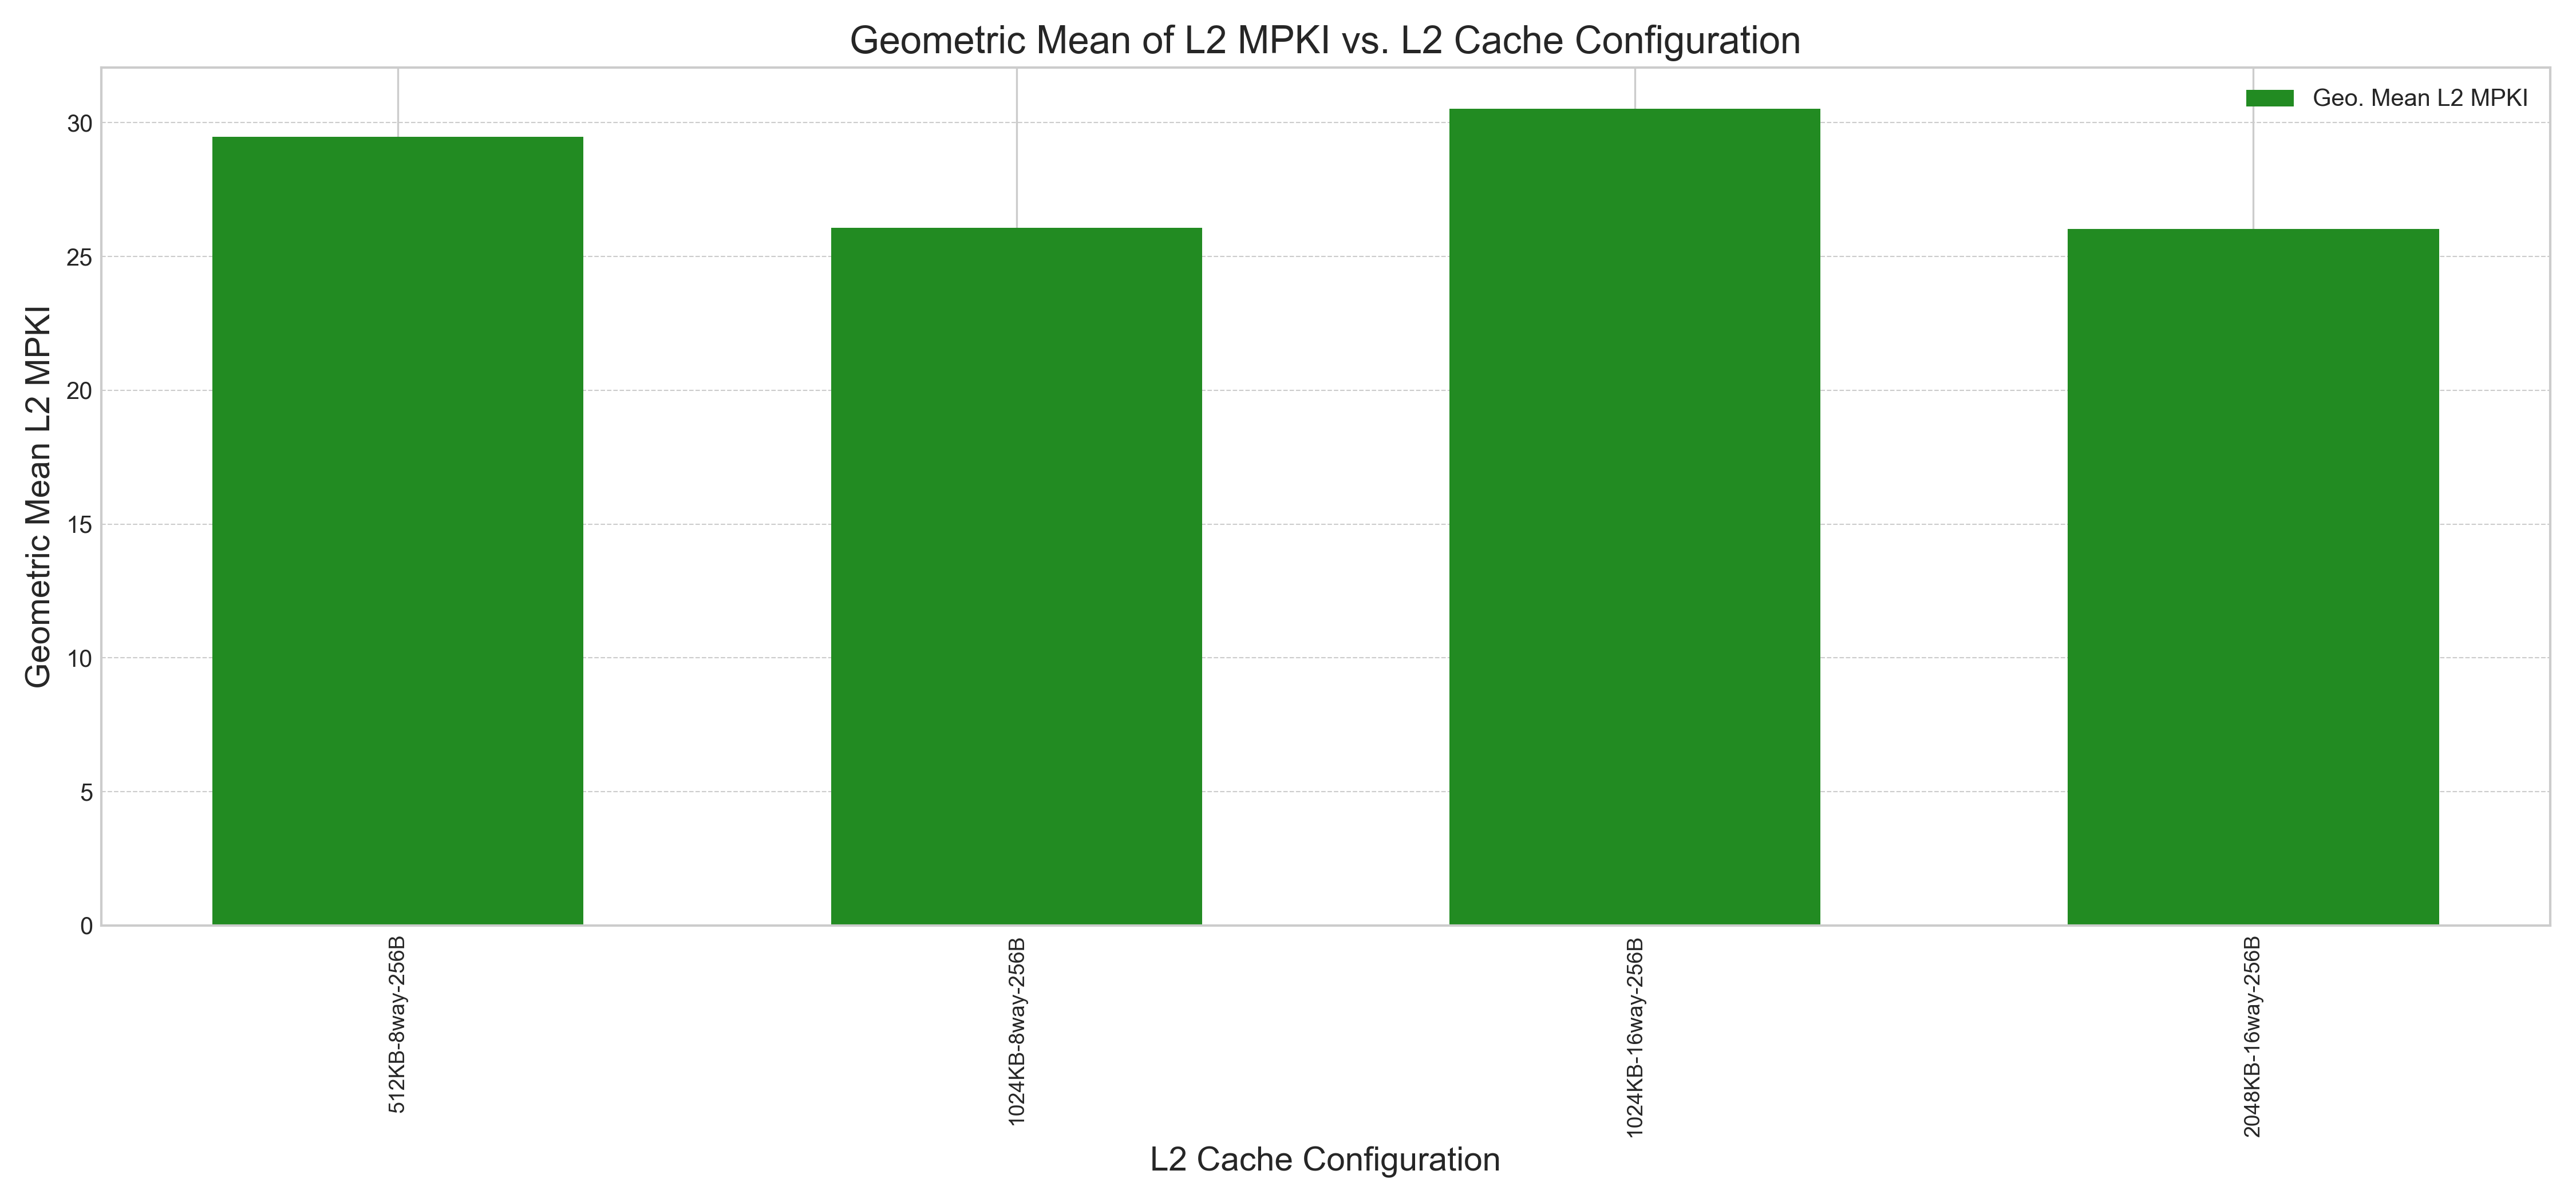
\includegraphics[width=0.8\textwidth]{figures/lfu/mpki_lfu.png}
    \caption{LFU Replacement Policy Results}
    \label{fig:lfu_mpki}
\end{figure}

\begin{figure}[H]
    \centering
    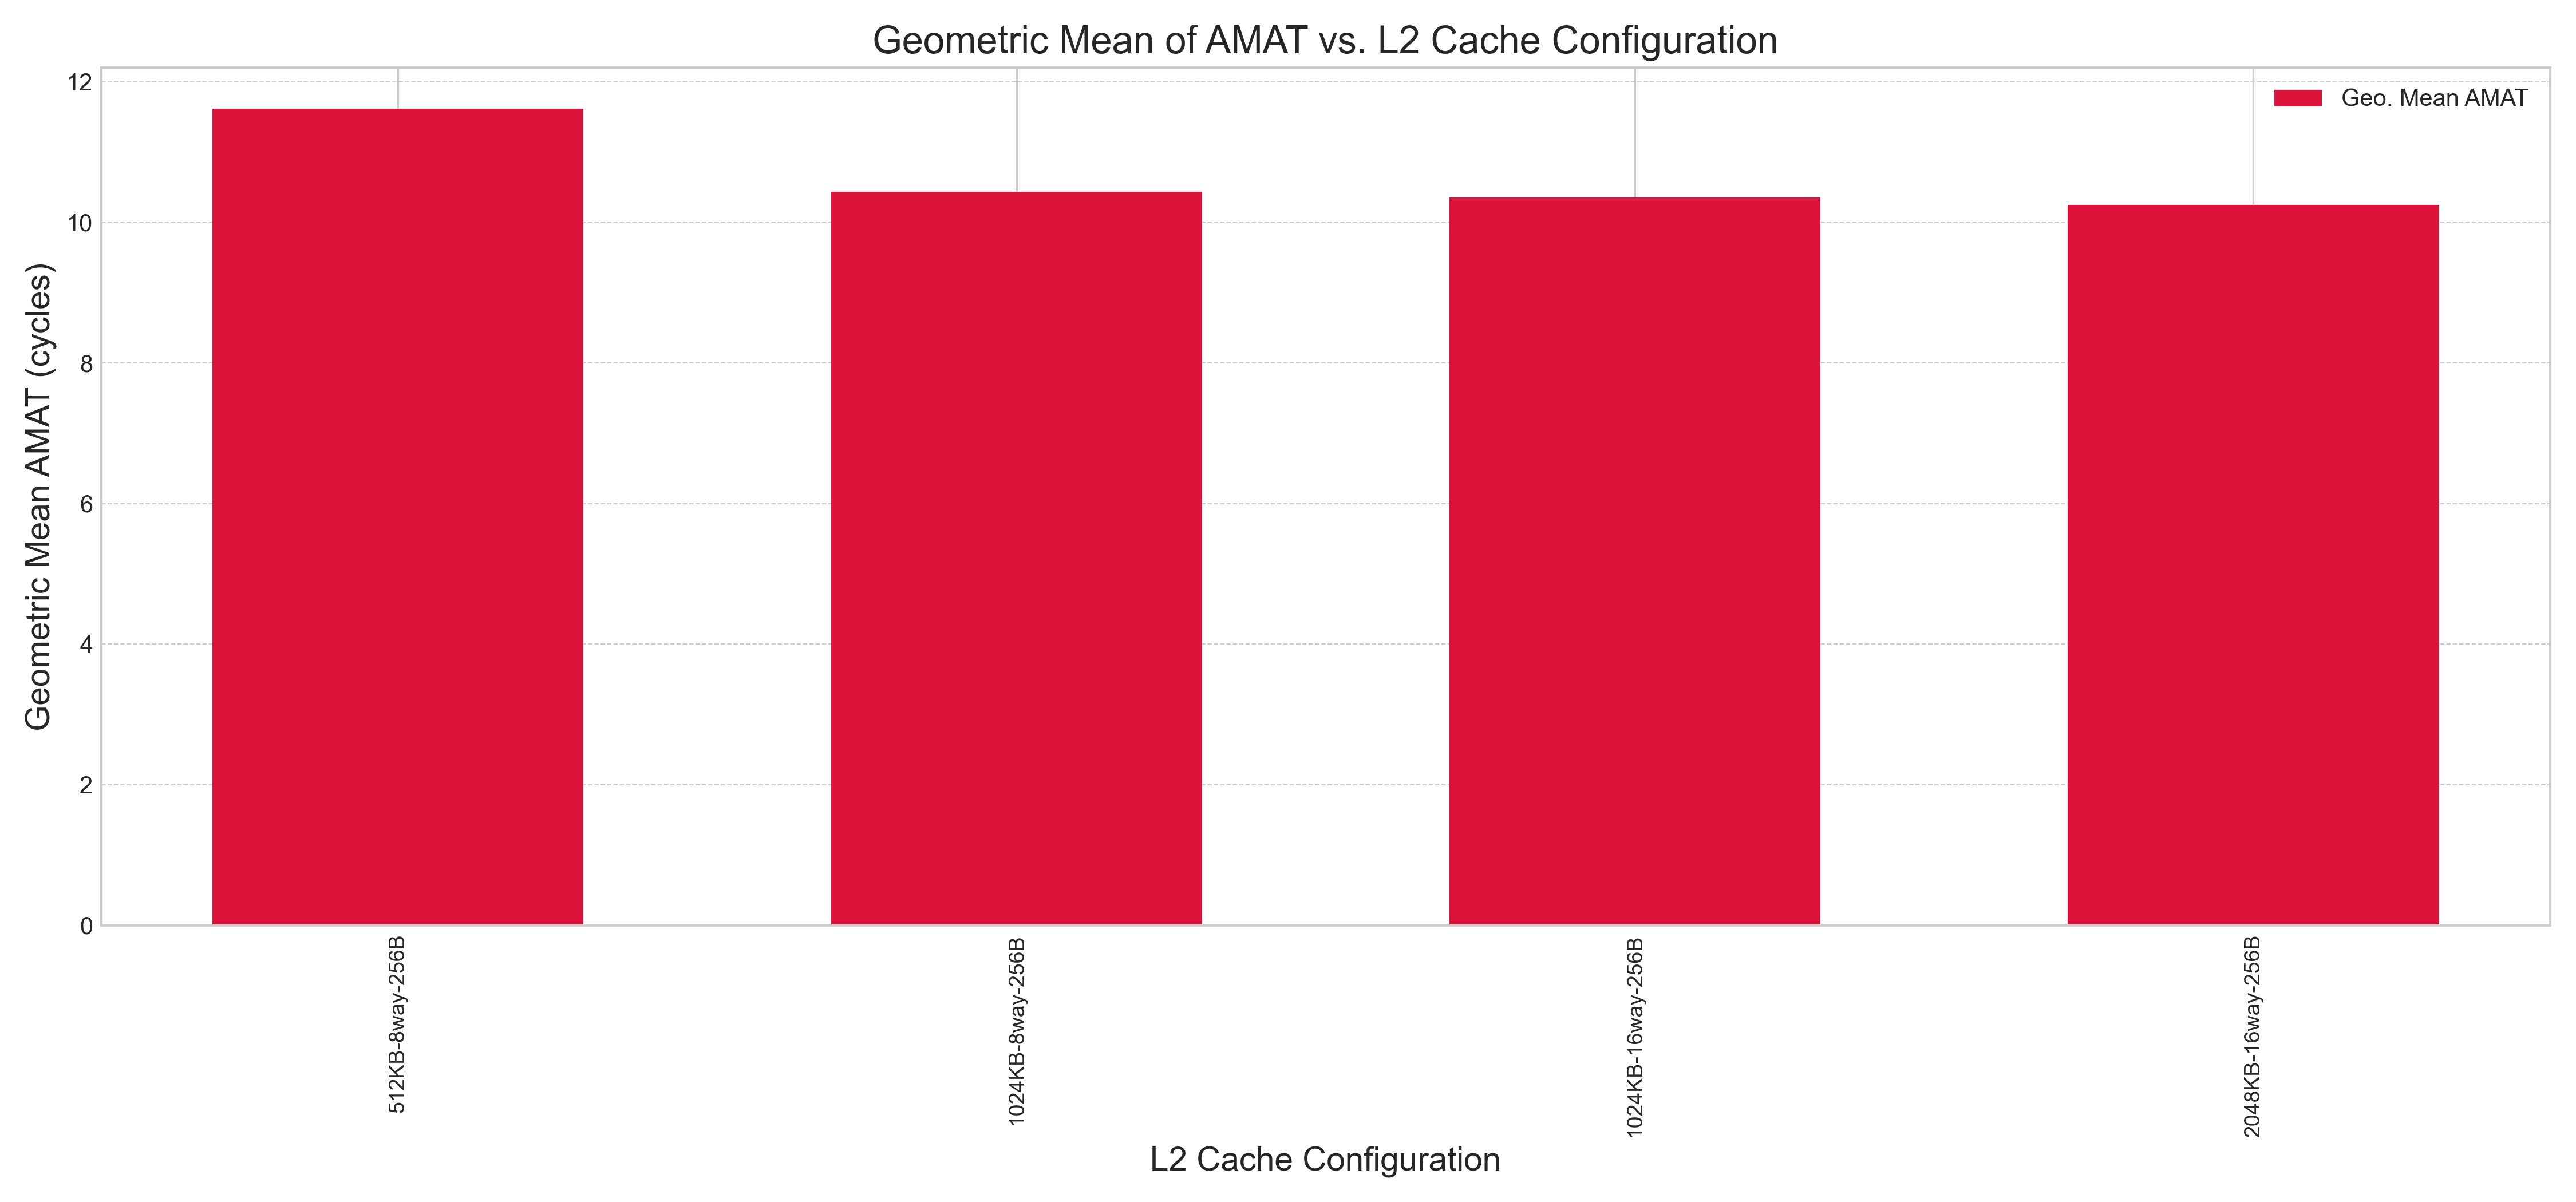
\includegraphics[width=0.8\textwidth]{figures/lip/amat_lip.png}
    \caption{LIP Replacement Policy Results}
    \label{fig:lip_amat}
\end{figure}

\begin{figure}[H]
    \centering
    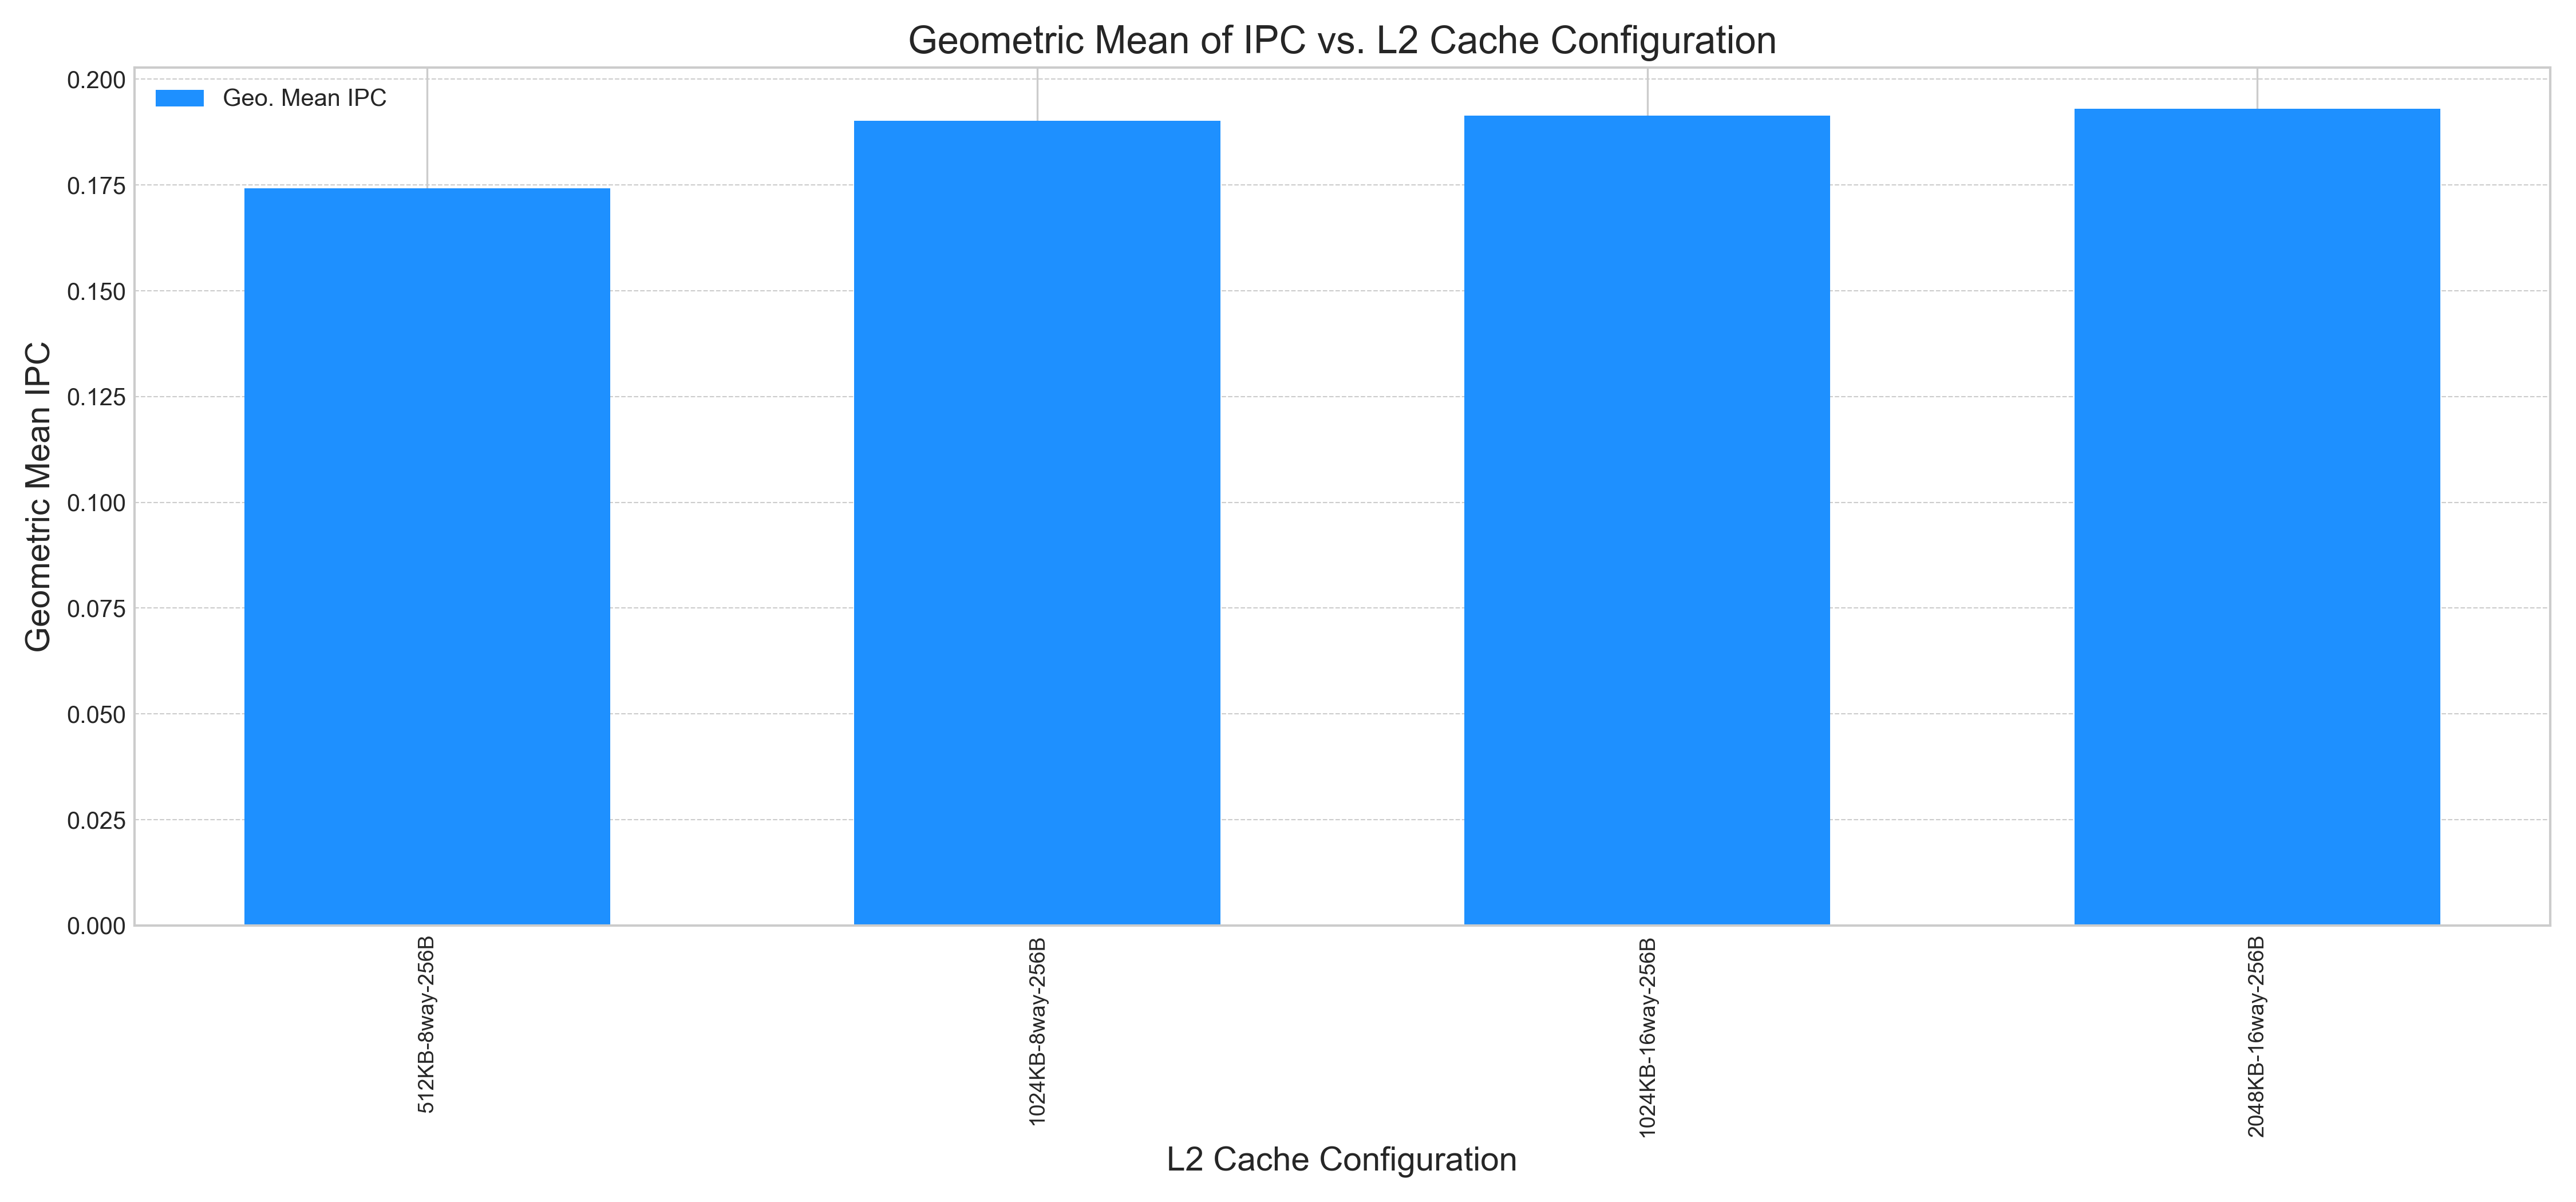
\includegraphics[width=0.8\textwidth]{figures/lip/ipc_lip.png}
    \caption{LIP Replacement Policy Results}
    \label{fig:lip_ipc}
\end{figure}

\begin{figure}[H]
    \centering
    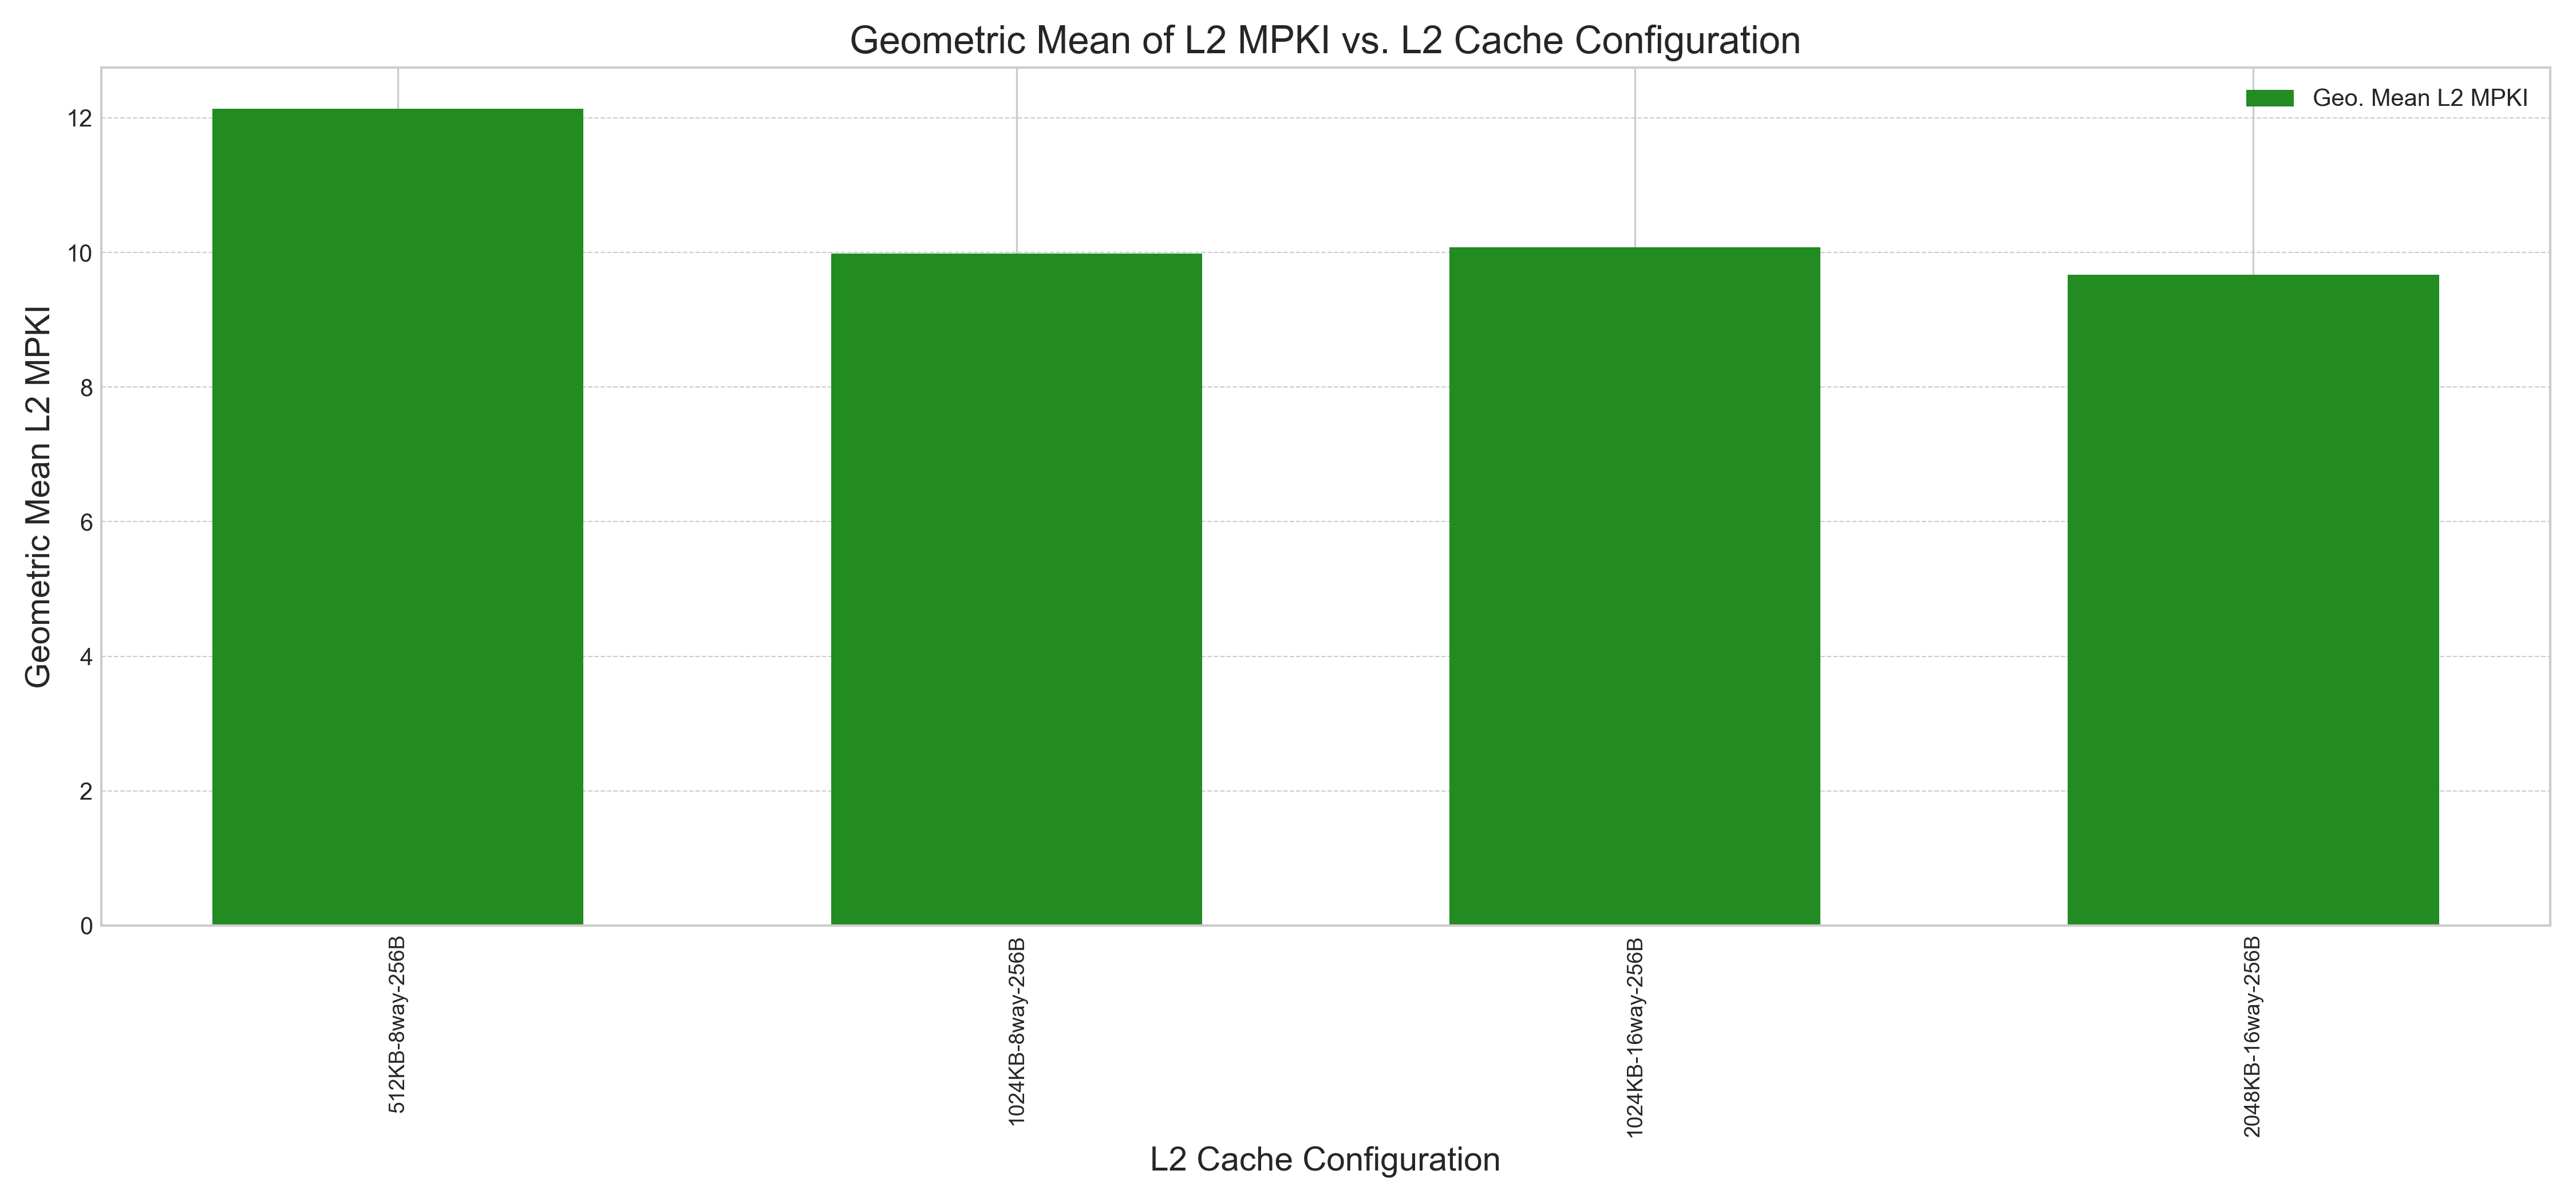
\includegraphics[width=0.8\textwidth]{figures/lip/mpki_lip.png}
    \caption{LIP Replacement Policy Results}
    \label{fig:lip_mpki}
\end{figure}

\begin{figure}[H]
    \centering
    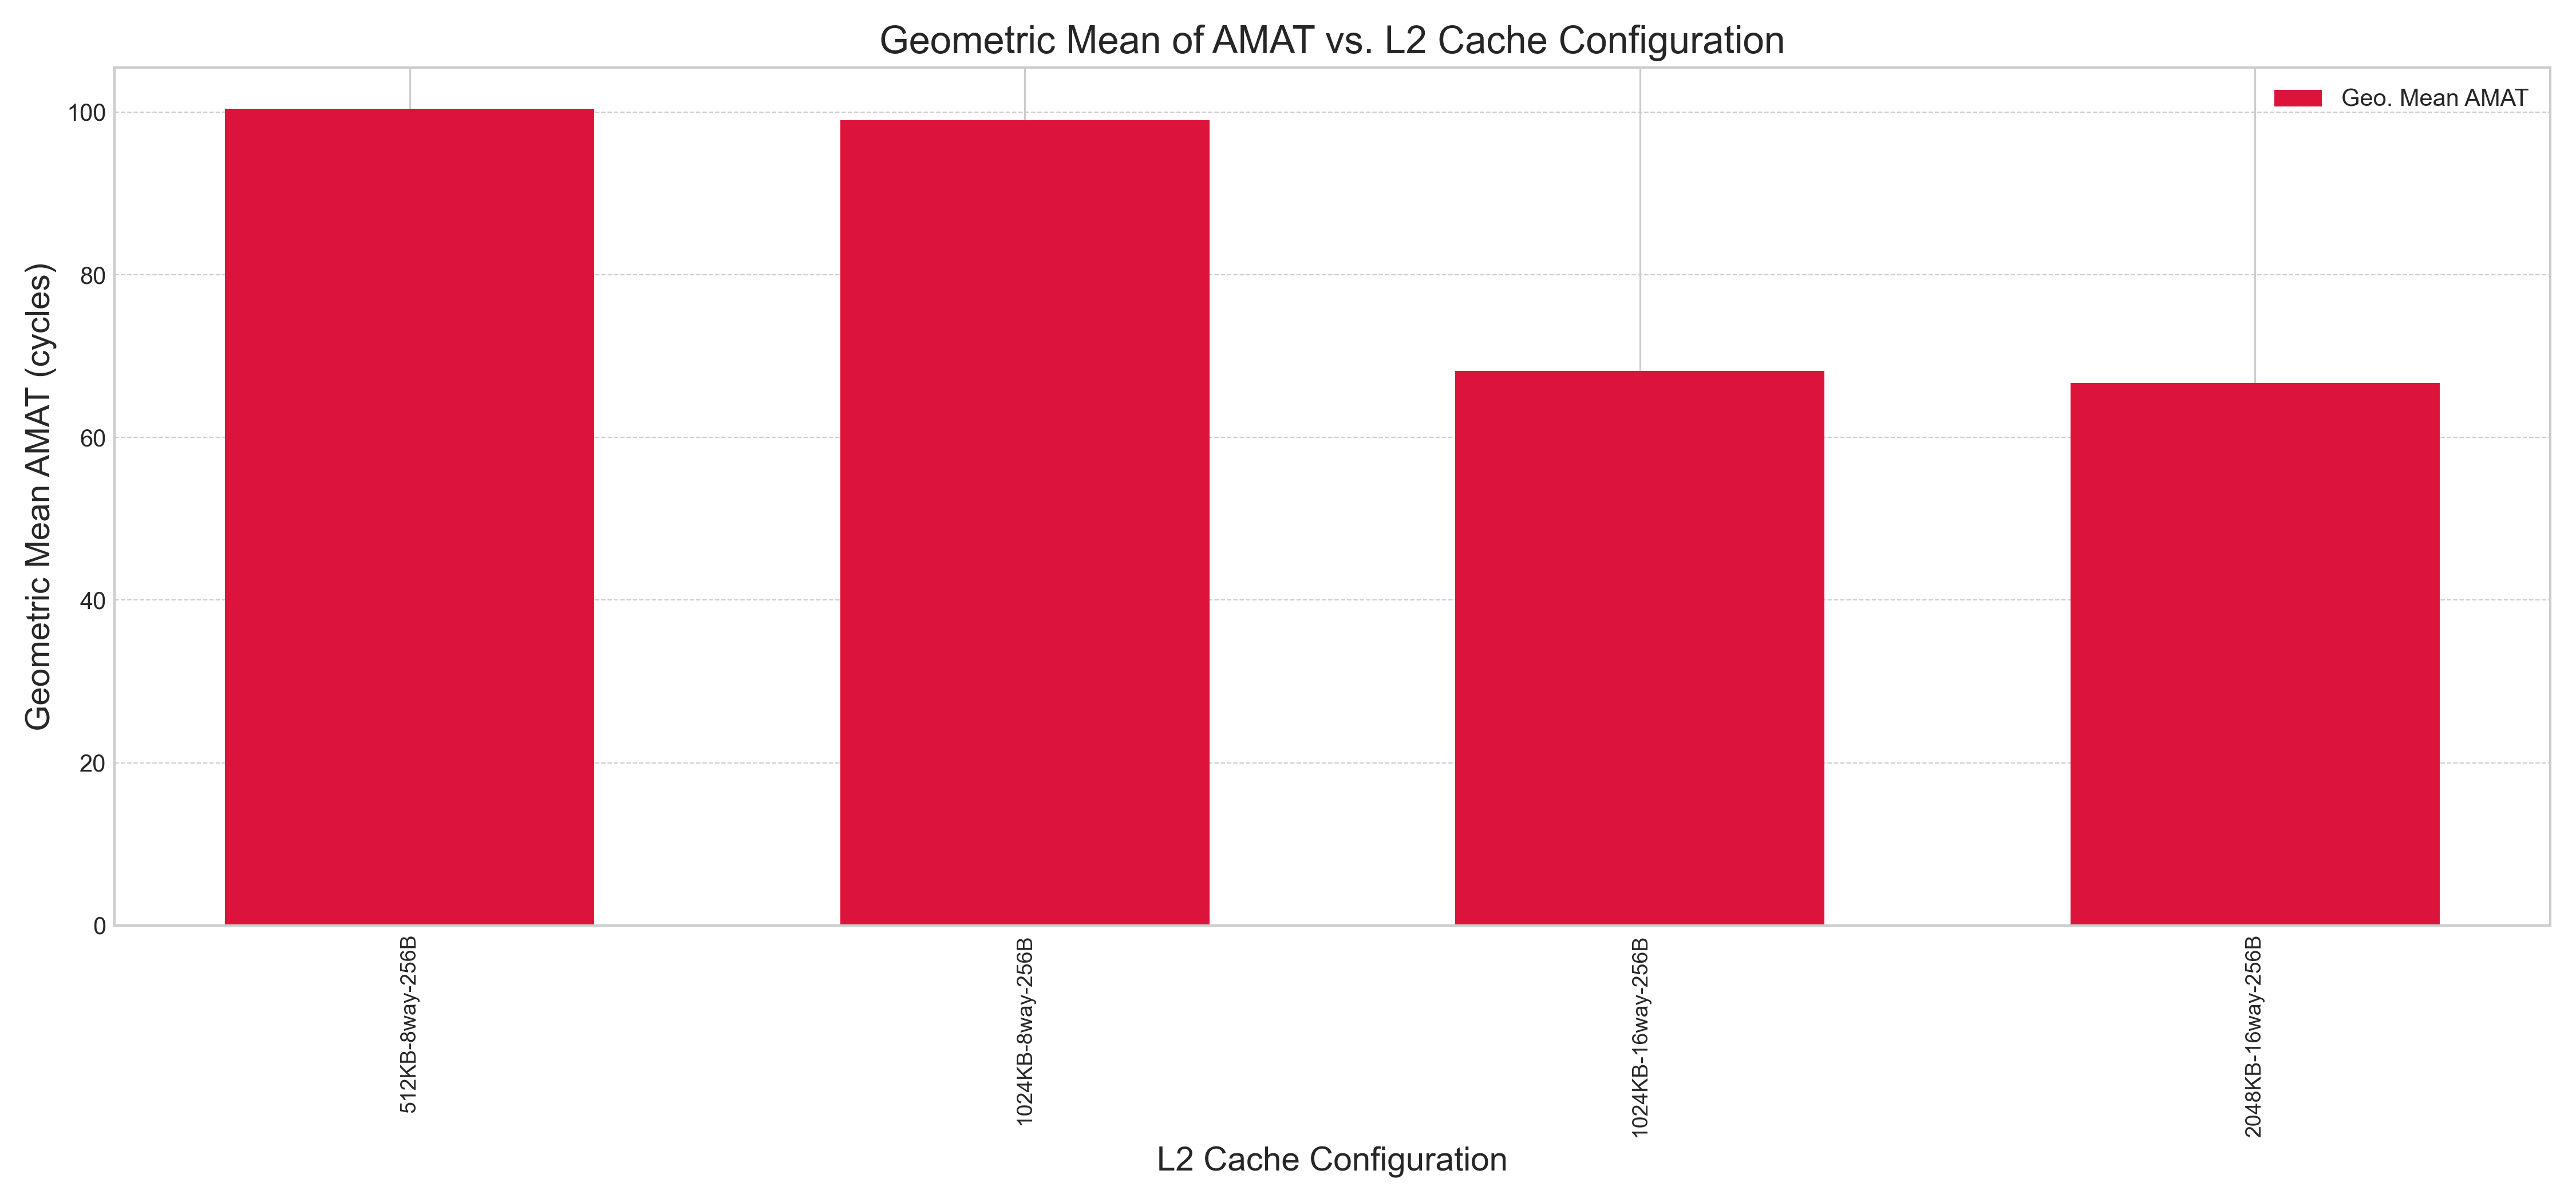
\includegraphics[width=0.8\textwidth]{figures/srrip/amat_srrip.png}
    \caption{SRRIP Replacement Policy Results}
    \label{fig:srrip_amat}
\end{figure}

\begin{figure}[H]
    \centering
    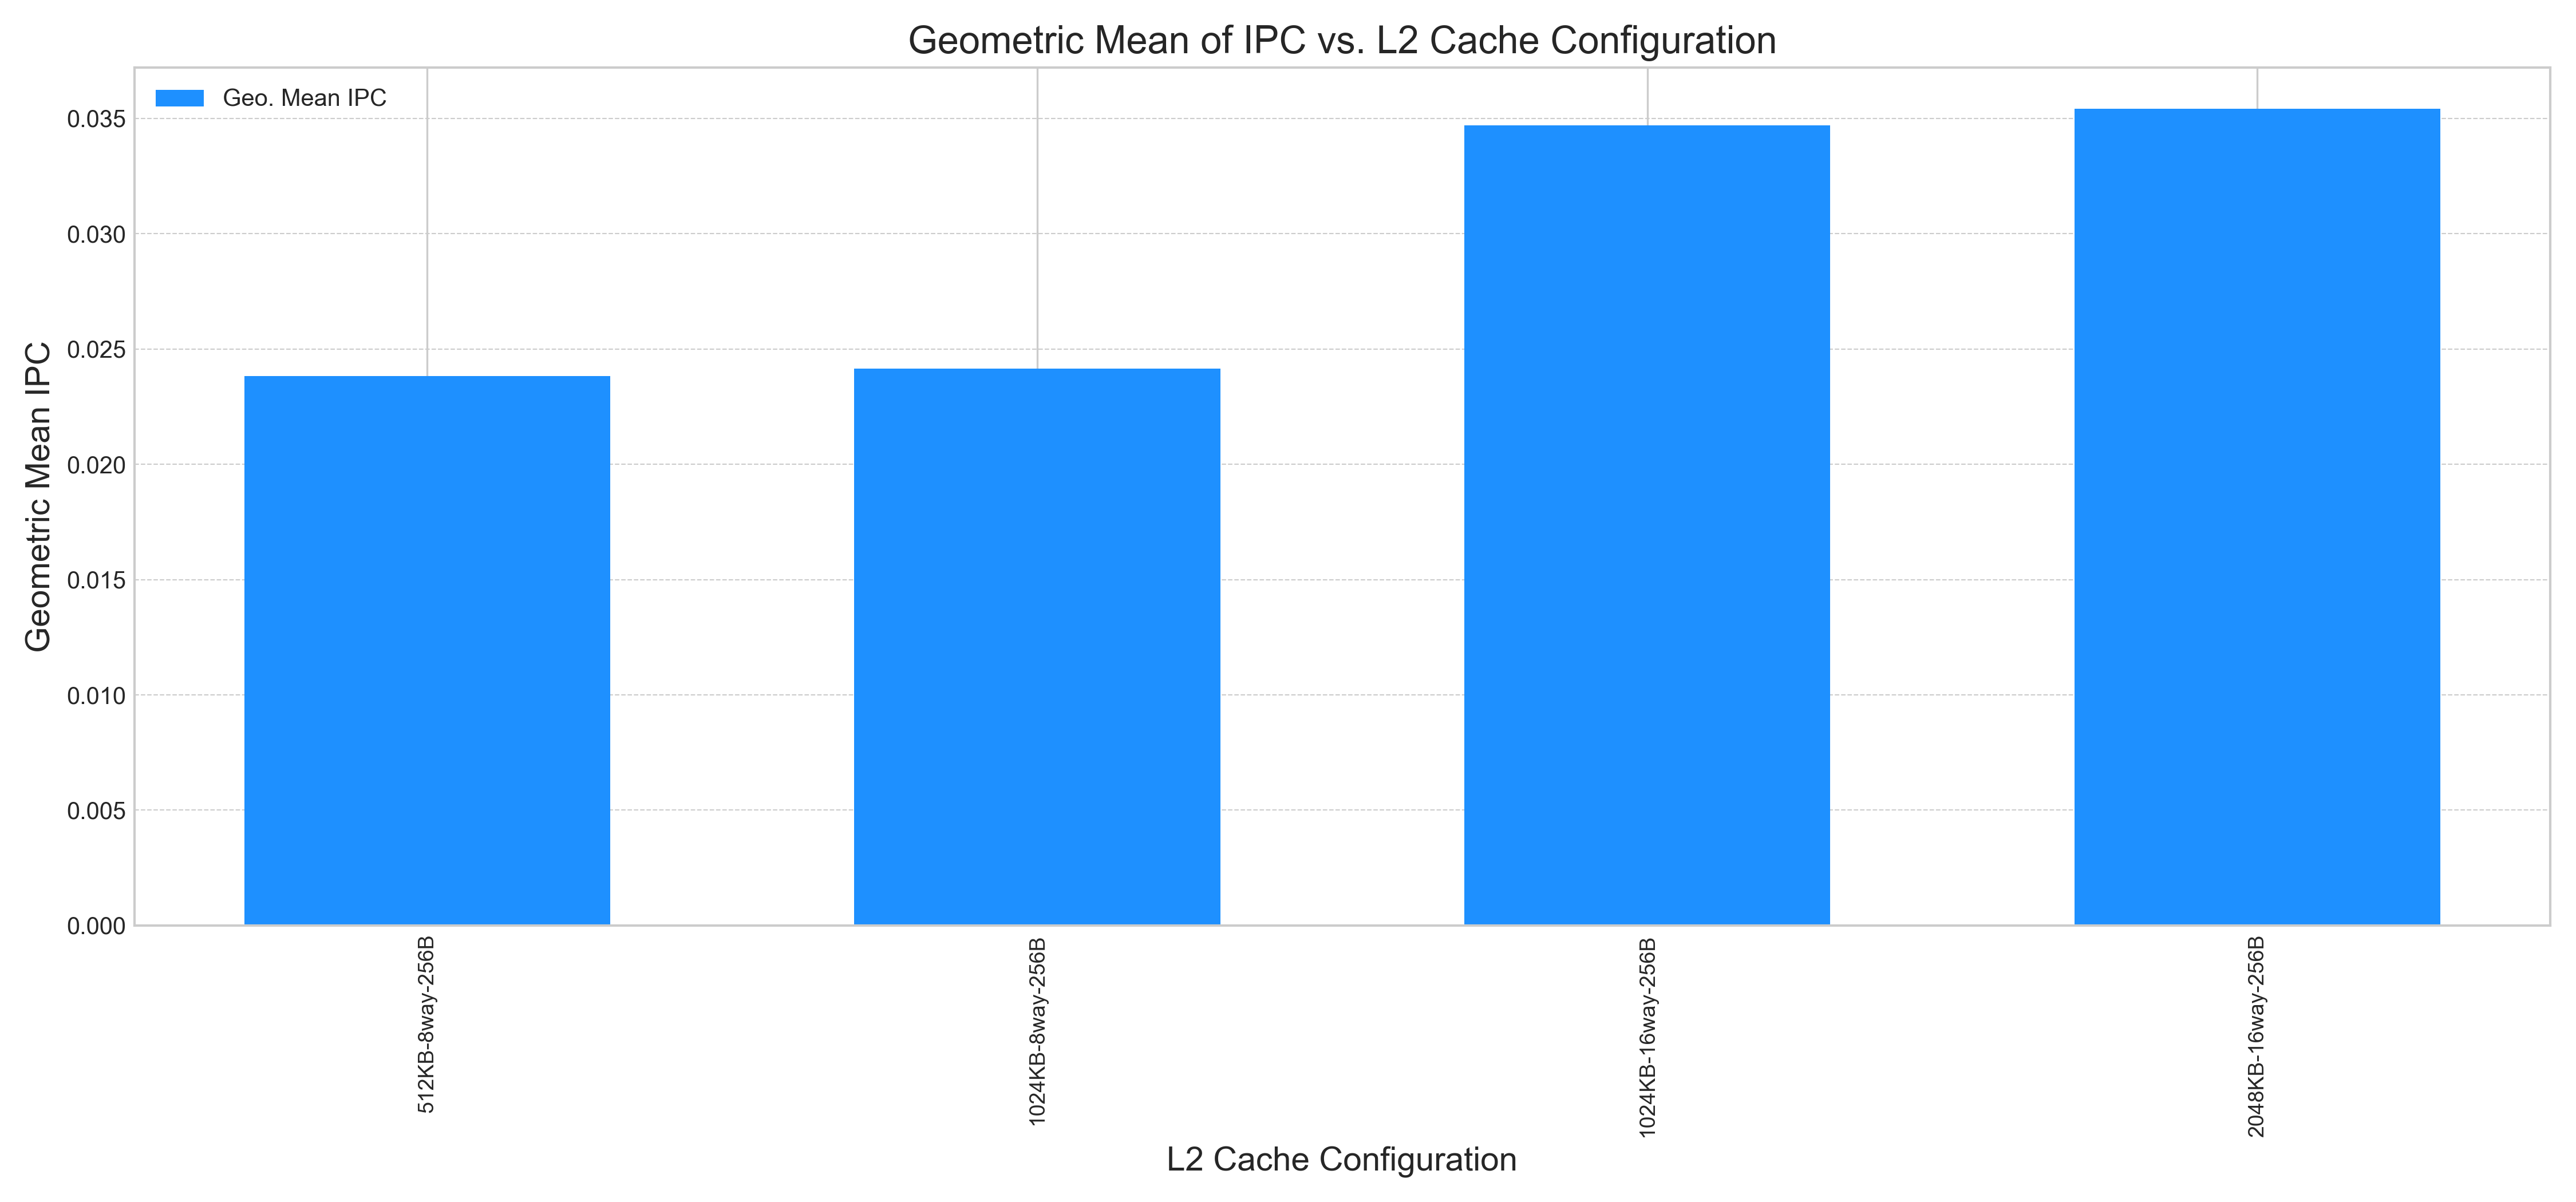
\includegraphics[width=0.8\textwidth]{figures/srrip/ipc_srrip.png}
    \caption{SRRIP Replacement Policy Results}
    \label{fig:srrip_ipc}
\end{figure}

\begin{figure}[H]
    \centering
    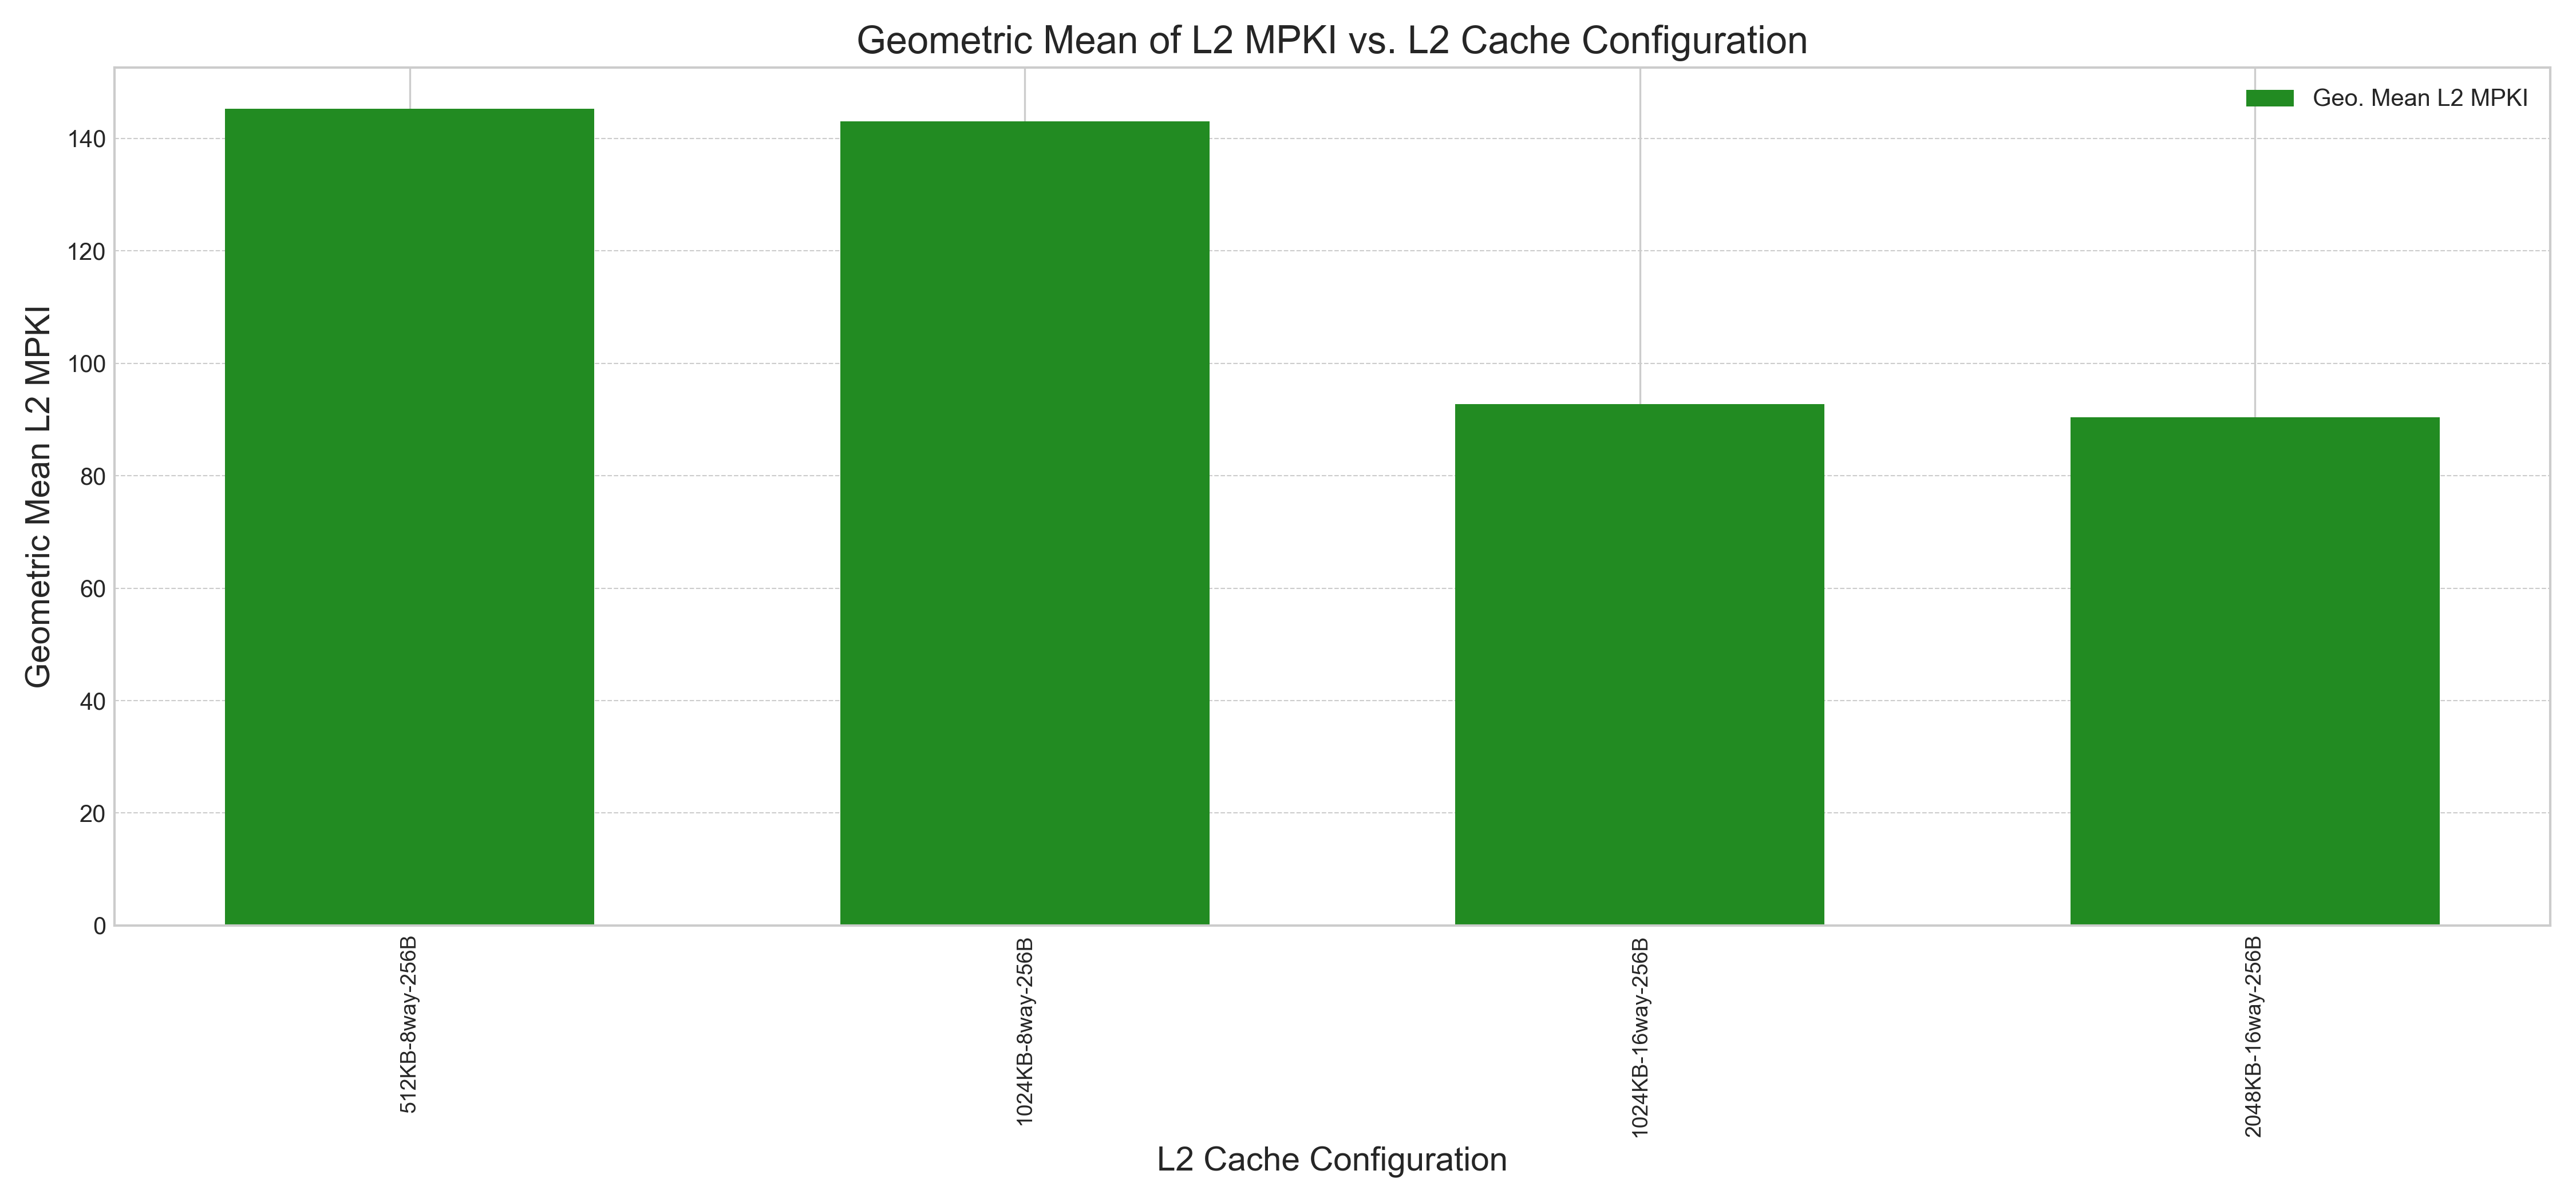
\includegraphics[width=0.8\textwidth]{figures/srrip/mpki_srrip.png}
    \caption{SRRIP Replacement Policy Results}
    \label{fig:srrip_mpki}
\end{figure}

Συγκρίνοντας τις πέντε πολιτικές αντικατάστασης (LRU, Random, LFU, LIP, SRRIP) βάσει των παραπάνω αποτελεσμάτων:

\begin{itemize}
    \item Η πολιτική \textbf{LRU} επιδεικνύει την καλύτερη συνολική απόδοση για τις εξεταζόμενες διαμορφώσεις L2 cache. Για παράδειγμα, για την διαμόρφωση C4 (2048KB-16way-256B), η LRU πετυχαίνει IPC $\sim 0.225$, AMAT $\sim 8.2$ cycles και L2 MPKI $\sim 8.0$. Αυτές οι τιμές είναι ανώτερες από όλες τις άλλες πολιτικές που δοκιμάστηκαν.
    \item Οι πολιτικές \textbf{Random} και \textbf{LIP} παρουσιάζουν την καλύτερη απόδοση μεταξύ των \textit{νέων} πολιτικών που υλοποιήθηκαν, με σχεδόν ταυτόσημες επιδόσεις μεταξύ τους. Για την C4, πετυχαίνουν IPC $\sim 0.205$, AMAT $\sim 9.2$ cycles και L2 MPKI $\sim 8.8$. Αν και καλές, υπολείπονται της LRU.
    \item Η πολιτική \textbf{LFU} έχει σημαντικά χαμηλότερη απόδοση από τις LRU, Random και LIP. Οι τιμές IPC είναι πολύ χαμηλές (της τάξης του $\sim 0.09$), το AMAT είναι υψηλό (της τάξης των $\sim 14-15$ κύκλων) και το L2 MPKI επίσης υψηλό (της τάξης των $\sim 15$).
    \item Η πολιτική \textbf{SRRIP}, όπως υλοποιήθηκε και δοκιμάστηκε βάσει των αποτελεσμάτων της αναφοράς, έδειξε την χειρότερη απόδοση με πολύ μεγάλη διαφορά. Οι τιμές IPC είναι εξαιρετικά χαμηλές ($\sim 0.03$), ενώ οι τιμές AMAT και L2 MPKI είναι πάρα πολύ υψηλές.
\end{itemize}

\textbf{Επιλογή Πολιτικής:}
Με βάση τα αποτελέσματα των προσομοιώσεων, η πολιτική \textbf{LRU (Least Recently Used)} θα ήταν η βέλτιστη επιλογή για υλοποίηση στο σύστημα. 
Παρέχει σταθερά την υψηλότερη απόδοση (υψηλότερο IPC, χαμηλότερο AMAT και L2 MPKI) σε σύγκριση με όλες τις άλλες πολιτικές.

Εάν η LRU δεν ήταν διαθέσιμη για κάποιο λόγο (π.χ., λόγω πολυπλοκότητας υλοποίησης σε ορισμένα σενάρια), τότε η πολιτική Random θα ήταν η επόμενη καλύτερη επιλογή λόγω της καλής της απόδοσης σε σχέση με την απλότητά της. 
Ωστόσο, εφόσον η LRU αξιολογήθηκε και αποδίδει καλύτερα, παραμένει η προτεινόμενη.

Τέλος, αξίζει να σημειωθεί, πως χρησιμοποιώντας τις πολιτκές LFU και LIP είχαμε πολύ ταχύτερες επιδόσεις.
Παρ'όλα αυτά, είναι δύσκολο να εξάγουμε συμπεράσματα για την απόδοση τους, καθώς ενδέχεται να επηρεάζονται από την αρχιτεκτονική του συστήματος καθώς και άλλους παράγοντες που σχετίζονται με το περιβάλλον εκτέλεσης.
\end{document}